\section{Statistical Interpretation}%
\label{sec:statistical_analysis}

The statistical interpretation of the search for resonant and non-resonant \HH
production proceeds using the methods introduced in
\Cref{sec:statistical_inference}. The main results of the analysis are upper
limits on the signal strength and cross section of SM~\HH production via \ggF
and VBF and upper limits on the cross section of resonant \HH production via
scalar, narrow-width resonances produced in \ggF.

This section is structured as follows:~First, the statistical model is
introduced in \Cref{sec:sig_bkg_model}. Second, the results of the search for
SM~\HH and resonant \HH production are presented in \Cref{sec:results_nonres}
and \Cref{sec:results_res}, respectively. Finally, the statistical
interpretation is concluded with an estimation of the statistical significance
of the largest excess observed in the search for resonant \HH production in
\Cref{sec:global_significance}.


\subsection{The Statistical Models}%
\label{sec:sig_bkg_model}

A separate statistical model is constructed for every signal hypothesis to be
probed. These models describe the distribution of event counts in bins of the
MVA discriminants in the SRs and \mll in the \ZHF~CR. They are built with
\textsc{HistFactory} (cf.~\Cref{sec:histfactory}) and include the signal and
background estimates, as well as the associated uncertainties, described in
previous sections. The discriminants used in all analysis channels are
summarised in~\Cref{tab:fitted_variable}.

\begin{table}[htbp]
  \centering
  \caption[Summary of the discriminants used in the SRs and \ZHF~CR.]{Summary of
    the discriminants used in the SRs and the \ZHF~CR. The search for resonant
    \HH production uses the PNN discriminant evaluated with a mass parameter set
    to the resonance mass under test.}%
  \label{tab:fitted_variable}

  \begin{tabular}{l@{\hskip 25pt}ccccc}
    \toprule
    & \multicolumn{4}{c}{Discriminant used in channel} \\
    \cmidrule{2-5}
    Search                  & \hadhad & \lephad SLT & \lephad LTT & \ZHF CR \\
    \midrule
    SM \HH production       & BDT & NN & NN & \mll \\
    Resonant \HH production & PNN(\mX) & PNN(\mX) & PNN(\mX) & \mll \\
    \bottomrule
  \end{tabular}
\end{table}

The POIs of the search for non-resonant \HH production are the total SM~\HH
production cross section via \ggF and VBF, \xsecggfvbf, and the corresponding
signal strength
\begin{align*}
  \mu = \frac{\xsecggfvbf}{\xsecggfvbf^{\text{SM}}}
  \qquad \text{with} \qquad
  \xsecggfvbf^{\text{SM}} = \SI{32.78}{\femto\barn}
  \,\text{,}
\end{align*}
which measures the cross section relative to the SM prediction from
Refs.~\cite{Grazzini:2018bsd,Dreyer:2018qbw}. Notably, the interpretation of the
SM~\HH search does not distinguish between the \ggF and VBF production modes.
In the search for resonant \HH production, the cross
section~$\sigma(pp \to X \to HH)$ is used as the POI. Moreover, SM~\HH
production is not considered as a background in the search for resonant \HH
production. In either case, free normalisation factors that scale the
contributions of \ZHF and \ttbar backgrounds in all channels are included in the
model. Lastly, statistical uncertainties on the background rates estimated using
finite samples of simulated events or CR data are implemented according to the
simplified Barlow--Beeston method~\cite{barlow1993,conway2011}.

% The cross sections are inclusive in the decay modes of the Higgs bosons and
% are determined from the measurement in the \bbtautau channel assuming Higgs
% boson branching ratios as predicted by the SM.

% The parameters of the model are inferred from observed or Asimov data using
% maximum likelihood estimation.

% The parameters of the models are inferred by maximising their likelihood
% functions for an observed or Asimov dataset. The main results are based on
% likelihood ratio tests of hypothesised values of the POIs. Unless otherwise
% noted, asymptotic approximations are used for the sampling distributions of
% the likelihood ratio test statistic.

The statistical models were scrutinised during their development by performing
fits to Asimov data, CR data, CR and SR data but blinding the signal-like
regions at high MVA score, and finally fits to observed data in all
regions. Alternative models that exclude certain SRs were investigated to
understand the effect of individual channels on the results. At every step, the
MLE of the model parameters, including the parameter errors and correlations,
were inspected to ensure that the model behaves as expected. During early stages
of the analysis, these checks informed the construction of the statistical
model. However, after unblinding of the SRs the model remained fixed to avoid
the introduction of biases.


\subsubsection{Binning of MVA Discriminants}%
\label{sec:binning_alg}

The signal sensitivity of the search depends on the binning used for the MVA
discriminants in the statistical interpretation. The binning has to be chosen
such that regions with high signal-to-background ratio (high MVA score) are
well-separated from regions with low signal-to-background ratio
(low/intermediate MVA score).

An iterative re-binning algorithm is used to determine the binning of the MVA
discriminants. The aim of the algorithm is to maximise the expected sensitivity
to a given signal while ensuring that the background prediction obeys
constraints on the statistical uncertainty and expected number of events in each
bin. These constraints ensure that asymptotic approximations can be used for the
statistical interpretation. The algorithm described in the following was
previously used in Ref.~\cite{HIGG-2016-16-witherratum} and is continued to be
used in the \hadhad channel of this search. In the \lephad channel, a minor
modification is applied to improve the signal sensitivity.
% A different, but conceptually similar algorithm is used in the \lephad
% channels, which is documented in Ref.~\cite{HDBS-2018-40}.

The algorithm is provided with MVA score histograms with fine, equidistant
binning separately for the signal and total background expectation at the
nominal values of all NPs. It proceeds by iteratively merging bins, starting
from the most signal-like MVA score bins, until the bin fulfils a set of
requirements:
\begin{enumerate}

\item The relative statistical uncertainty of the background prediction in the
  bin must be smaller
  than~\mbox{$\SI{50}{\percent} \times f_\text{s} + \SI{1}{\percent}$}, where
  $f_\text{s}$ is the fraction of signal events in the bin with respect to the
  total number of signal events selected in the channel. This requirement limits
  the statistical uncertainty of the background estimate in the most signal-like
  bins to be in a range of \SIrange{10}{20}{\percent} after re-binning.

  In the \lephad channel, a requirement of
  $10 f_{\text{s}} + 5 f_{\text{b}} > 1$ is used instead, where $f_{\text{b}}$
  is the fraction of background events defined in analogy to~$f_{\text{s}}$.

  % \footnote{In the \lephad
  %   channels, a requirement of $10 f_{\text{s}} + 5 f_{\text{b}} > 1$ is used
  %   instead, where $f_{\text{b}}$ is the fraction of background events defined
  %   in analogy to~$f_{\text{s}}$.}

\item The expected number of background events in the bin must be larger than
  five.

\end{enumerate}
When a bin fulfilling all requirements is found, the process is repeated
starting from the next bin that is not yet merged. The algorithm terminates with
a final bin at low MVA score. If the final bin does not fulfil the criteria, it
is merged with the preceding bin.
% In the \lephad channels, the requirements for bins are altered to at least
% five expected background events and $10 f_{\text{s}} + 5 f_{\text{b}} > 1$,
% where $f_{\text{b}}$ is the fraction of background events defined in analogy
% to~$f_{\text{s}}$.
The size of bins resulting from the re-binning procedure can vary by multiple
orders of magnitude. For visualisation purposes, the variable-width MVA score
bins are therefore displayed as equidistant bins.


% \subsubsection{Merging of Physics Processes}

% The statistical models are simplified by merging samples originating
% from similar underlying physics processes which are subject to equal
% treatment in the fit model. In the SM \HH search, the \ggF and VBF
% samples are merged, defining the total signal contribution from both
% production modes. The \Zjets samples are combined into
% $Z + (bb,bc,cc)$ and $Z + (bl,cl,ll)$ samples, separately for
% $Z \to \tau\tau$ and $Z \to \ell^+\ell^-$, where $\ell = e,
% \mu$. Further, contributions from diboson and single top production
% (including $tW$) are merged into two separate samples.

% The treatment merging for \faketauhadvis backgrounds differs between
% the \hadhad and \lephad channels. In the \hadhad channel two separate
% samples are used for \tauhadvis background from multi-jet and \ttbar
% production. In \lephad channels, all \faketauhadvis contributions are
% merged since the estimation method does not distinguish between the
% \faketauhadvis source.

% The merging of samples should not have a large effect on the
% statistical analysis. The only differences arise from symmetrisation,
% smoothing, and pruning algorithms (discussed in the following) acting
% on merged samples instead of the initial components.


\subsubsection{Symmetrisation of Systematic Uncertainties}

Uncertainties derived from comparisons of the nominal with an alternative
prediction only provide a single systematic variation and cannot be readily
incorporated in the statistical model. In this case, variations are symmetrised
by mirroring their effect with respect to the nominal prediction.

Uncertainties with up- and down-variations that change the prediction in one or
multiple bins in the same direction are also subject to symmetrisation. Such
variations usually result from statistical fluctuations and can lead to
artificial over- or underconstraints of the associated NPs after the fit.
% \footnote{Overconstrained (underconstrained) NPs are parameters with post-fit
% uncertainties that are smaller (larger) than the pre-fit uncertainty of the
% parameter. They are referred to as ``artificial'' since they arise from a
% mis-specification of the model as opposed to physical reasons.}
In this case, uncertainties are symmetrised by assigning half of the difference
between the up- and down-variation as a symmetric uncertainty. This
symmetrisation method is selectively applied to affected uncertainties, such as
the jet energy scale and resolution uncertainties.

% \subsubsection{Inter- and Extrapolation of Systematic Uncertainties}

% To define a continuous likelihood function, the effects of nuisance
% parameters on the signal and background expectations have to be
% parameterised as continuous functions of the
% parameters. Uncertainties are typically defined by an up- and
% down-variation and the nominal prediction which correspond to
% nuisance parameter values of $\alpha = \pm 1$ and $\alpha = 0$,
% respectively.

% The parametrisation is obtained by interpolation
% ($\vert \alpha \vert \leq 1$) and extrapolation
% ($\vert \alpha \vert > 1$) methods provided by
% \textsc{HistFactory}~\cite{cranmer2012}.

% All uncertainties are split into uncertainties only affecting the
% normalisation and uncertainties only affecting the shape of
% distributions. Both components are considered as fully correlated in
% the model. Different inter- and extrapolation methods are used for
% normalisation and shape uncertainties.

% All uncertainties are decomposed into two correlated components
% employing different inter- and extrapolation methods. The first
% component are uncertainties on the sample normalisations in a given
% region which are parameterised using multiplicative normalisation
% factors determined from 6th order polynomial interpolation and
% exponential extrapolation in $\alpha$. Exponential extrapolation is
% used to prevent the normalisation factors from becoming negative. The
% second component are shape variations of the discriminant in a given
% region that leave the normalisation invariant. The parameterised shape
% variations are obtained using 6th order polynomial interpolation and
% linear extrapolation. In both cases, the resulting functions are
% required to be continuous and have continuous first and second
% derivatives at the boundaries.

% Normalisation uncertainties use 'FlexibleInterpVar' in HistFactory
% with code 4 (polynomial interpol and exponential extrapol).
%
% Shape uncertainties use 'PiecewiseInterpolation' in HistFactory with
% code 4 (polynomial interpolation and linear extrapolation)


\subsubsection{Smoothing and Pruning of Systematic Uncertainties}

% https://indico.cern.ch/event/736395/contributions/3040869/attachments/1671620/2684026/SmoothingPruning.pdf
% https://cds.cern.ch/record/2692202/files/CERN-THESIS-2018-447.pdf
All uncertainties are split into separate normalisation and shape uncertainties
that are correlated in the statistical model. The templates used to define shape
uncertainties are susceptible to statistical fluctuations, which can introduce
spurious pulls or constraints of NPs after the fit. This is often the case when
deriving shape uncertainties from a two-sample comparison or from variations
that change the four-momentum of reconstructed physics objects. In these cases,
a smoothing procedure is applied that is adopted from
Ref.~\cite{HIGG-2013-23}. Shape uncertainties based on a re-weighting of the
nominal prediction are less susceptible to statistical fluctuations and thus no
smoothing is applied by default. An exception is made for the variations of the
final-state radiation in single top-quark and \ttbar production. These are
subject to large statistical fluctuations and are therefore smoothed.

% The derivation of shape uncertainties are susceptible to statistical
% fluctuations\footnote{This is can also be the case for normalisation
%   uncertainties which are not the subject of the smoothing
%   algorithm. In this case the user is responsible to ensure that
%   normalisation uncertainties are determined with sufficient
%   precision.} which can introduce spurious pulls and constraints on
% nuisance parameters when performing maximum likelihood fits of the
% model. Frequently this is the case when shape uncertainties are
% derived from MC-to-MC comparisons or from variations that change the
% four-momentum of final state particles. In these cases a smoothing
% procedure is applied to the templates describing the uncertainties on
% the shape of the discriminant. Shape uncertainties that are based on
% the re-weighting of the nominal prediction are less sensitive to
% statistical fluctuations, unless the weight distribution has high
% variance, and thus no smoothing is applied by default. Exceptions are
% made in some cases for example for the weight-based FSR uncertainties
% for the production of top-quarks for which smoothing is applied due to
% the large variance of the associated weight distribution.

% The smoothing procedure, adopted from Ref.~\cite{HIGG-2013-23}, uses
% iterative re-binning of the histogram-based templates describing the
% shape uncertainties, merging bins starting with bins that are most
% compatible until the statistical uncertainty in all bins is below
% \SI{5}{\percent} and the shape template has a monotonic
% dependency\todo{Why?} on the (MVA) discriminant. This procedure is
% applied, when configured for a given uncertainty, separately for all
% analysis regions and samples after merging.

After symmetrisation and smoothing, the model is simplified by removing
(pruning) small systematic uncertainties. This procedure is applied separately
to all samples and channels, and separately for the normalisation and shape
components of uncertainties. The normalisation component of an uncertainty is
removed if both the up- and down-variation change the normalisation by less than
\SI{0.5}{\percent}. The shape component of an uncertainty is removed if the
relative change of the up- and down-variations in all bins of a given channel is
less than \SI{0.5}{\percent}.


\subsubsection{Nuisance Parameter Correlation Scheme}

All normalisation factors are correlated between channels. NPs related to
instrumental uncertainties are correlated between all channels and physics
processes. Theory uncertainties on cross sections and acceptances for a given
process are assumed to be correlated between channels provided they originate
from the same source. NPs related to the \faketauhadvis background estimation
are not correlated between the \hadhad and \lephad channels since different
estimation methods are used. However, they are correlated between the \lephad
SLT and LTT channel, which use the same estimation techniques.

An exception to this scheme are the parton shower uncertainties for \ttbar which
were decorrelated between the \hadhad, \lephad SLT, and \lephad LTT
channel. This decision is based on observed tensions between the best-fit NP
values when performing fits of the individual channels.

% Hadhad: No pull, slight overconstraint
% Lephad SLT: Large overconstraint
% Lephad LTT: Pull and overconstraint


\subsection{Results of the Search for SM~\HH Production}%
\label{sec:results_nonres}

The results of the search for SM~\HH production are presented for the
combination of all channels. Results are also presented prior to the combination
of the \hadhad and \lephad channels to illustrate the signal sensitivity of
individual channels and differences in the impact of systematic uncertainties.
% Unless otherwise noted, all results are obtained from the model using the
% SM~\HH signal strength as the POI.
Selected background processes are merged for illustration purposes only. The
contributions from \ttbar and single top-quark production are combined into a
``top-quark'' background category. Contributions from minor backgrounds are
combined into the ``other'' background category, which includes
$Z \to \tautau + \text{LF}$, $Z \to e^{+}e^{-}$, $Z \to \mu^{+}\mu^{-}$, \Wjets,
diboson, and $\ttbar V$.

The background-only model is fitted to observed data in all
channels. \Cref{fig:mvascores_postfit} compares the post-fit MVA score
distributions in the three SRs to data. The post-fit prediction describes the
observed data in the SRs well. In addition, the expected event yields per
process in the SRs after the maximum likelihood fit are summarised
in~\Cref{tab:postfit_yields_smhh}. Finally, the normalisation factors of \ttbar
and \ZHF resulting from the fit are \num{0.97 +- 0.04} and \num{1.40 +- 0.11},
respectively, which are consistent with the results obtained from fits
restricted to the \ZHF~CR in~\Cref{sec:bkg_zjets}.
%%%%%%%%%%%%%%%%%%%%%%%%%%%%%%%%%%%%%%%%%%%%%%%%
% ATLAS_norm_Zhf      1.4021e+00 +/-  1.11e-01 %
% ATLAS_norm_ttbar    9.7030e-01 +/-  3.76e-02 %
%%%%%%%%%%%%%%%%%%%%%%%%%%%%%%%%%%%%%%%%%%%%%%%%

\begin{figure}[htbp]
  \centering

  \begin{subfigure}{0.495\textwidth}
    \centering

    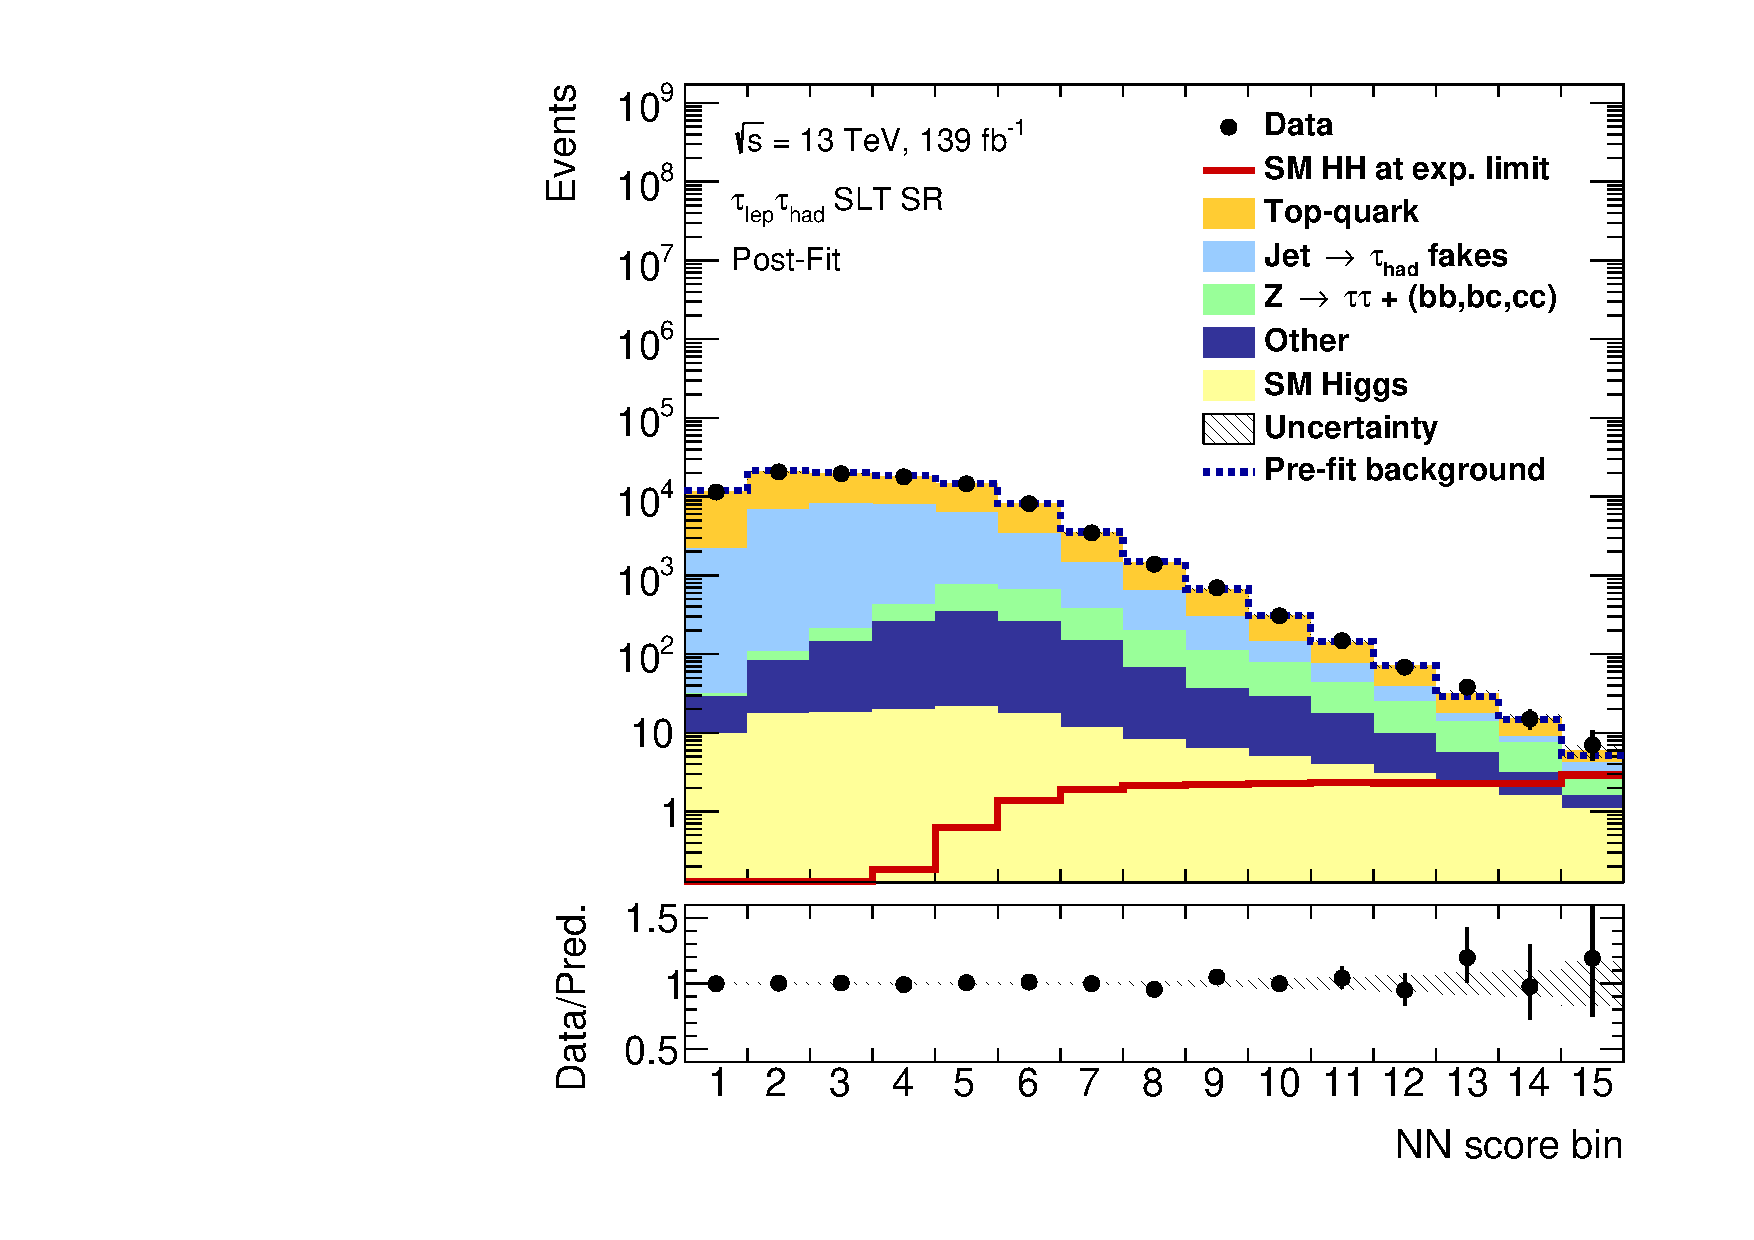
\includegraphics[width=\textwidth]{results_nonres/postfit/Region_BMin0_incJet1_distNN_J2_DSM_T2_SpcTauLH_Y2015_LTT0_L1_GlobalFit_conditionnal_mu0log}

    \subcaption{\lephad SLT channel}
  \end{subfigure}\hfill%
  \begin{subfigure}{0.495\textwidth}
    \centering

    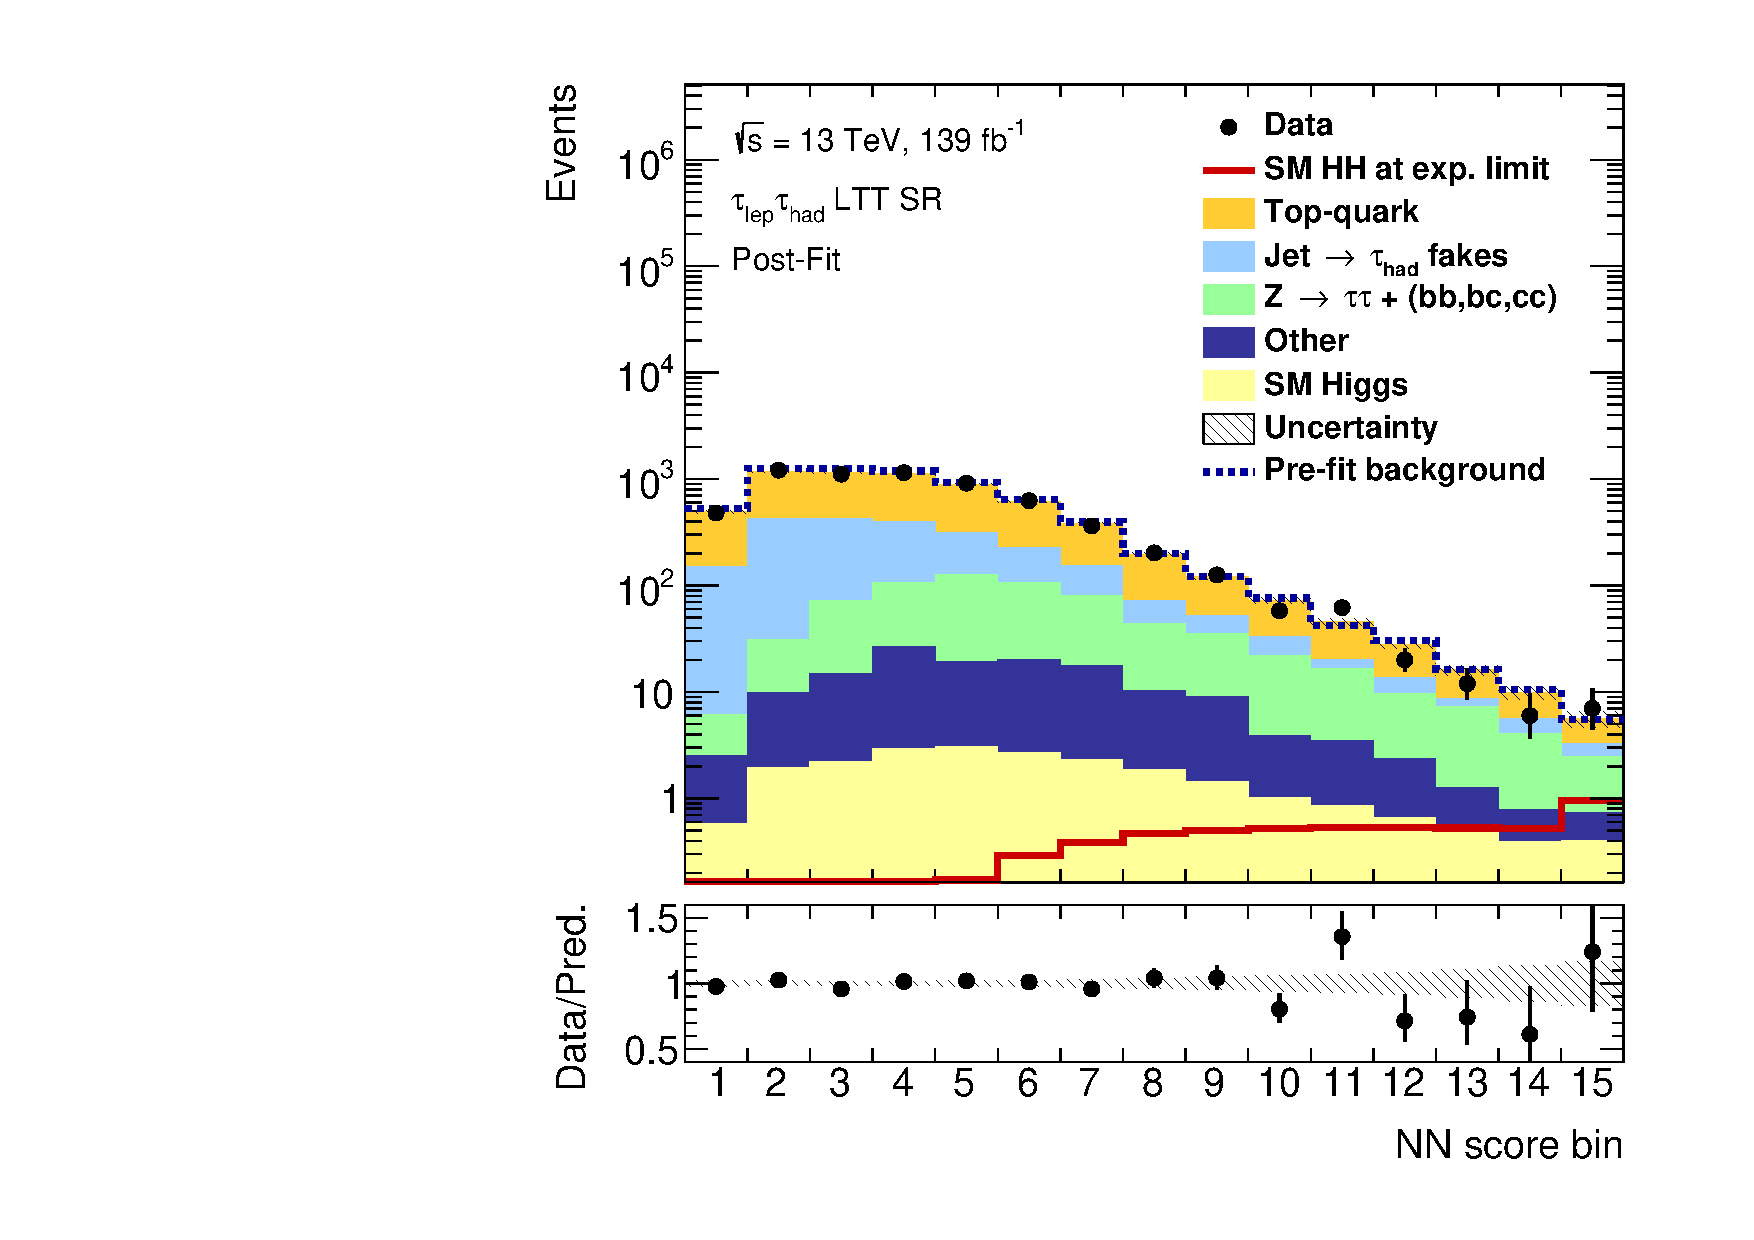
\includegraphics[width=\textwidth]{results_nonres/postfit/Region_BMin0_incJet1_distNN_J2_DSM_T2_SpcTauLH_Y2015_LTT1_L1_GlobalFit_conditionnal_mu0log}

    \subcaption{\lephad LTT channel}
  \end{subfigure}

  \vspace{0.5em}

  \begin{subfigure}{0.495\textwidth}
    \centering

    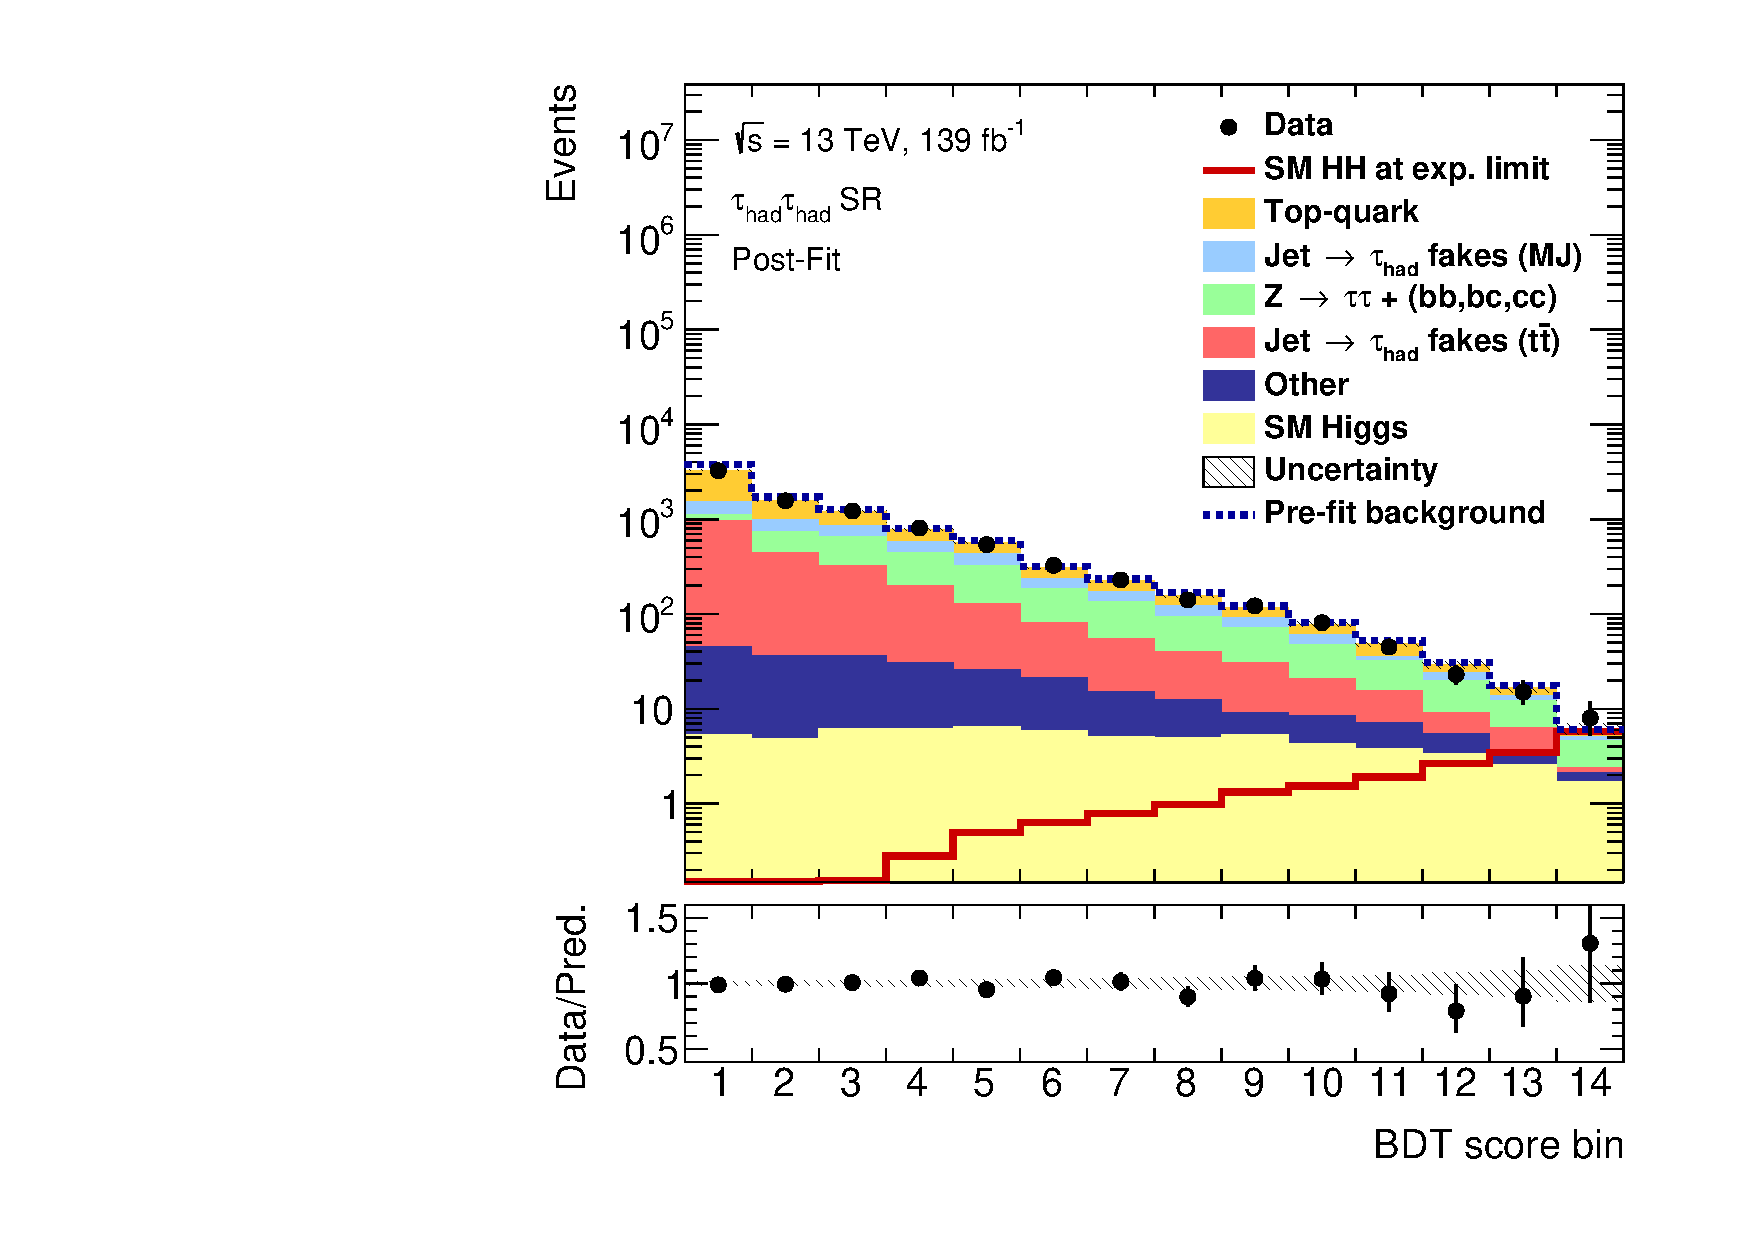
\includegraphics[width=\textwidth]{results_nonres/postfit/Region_BMin0_incJet1_distSMBDT_J2_Y2015_DLLOS_T2_SpcTauHH_L0_GlobalFit_conditionnal_mu0log}

    \subcaption{\hadhad channel}
  \end{subfigure}

  \caption[Distributions of the MVA discriminants used for the SM~\HH search
  after the background-only fit.]{Distributions of the MVA discriminants used
    for the SM~\HH search in the \lephad~SLT~(a), \lephad~LTT~(b), and
    \hadhad~(c) channel after the fit of the background-only model to observed
    data in all regions. The signal overlay is scaled to the expected upper
    limit on the signal strength of $3.9$ from the combination of all
    channels. The \faketauhadvis background in the \hadhad channel is shown
    separately for \faketauhadvis from multi-jet (MJ) and \ttbar.}%
  \label{fig:mvascores_postfit}
\end{figure}

\begin{table}[htbp]
  \centering

  \caption[Event yields in the three SRs and in the two most signal-like bins of
  the MVA discriminants after the background-only fit.]{Event yields in the
    three SRs (a) and in the two most signal-like bins of the MVA discriminants
    (b) after the background-only fit to the observed data in all regions. The
    category ``other backgrounds'' combines minor contributions from
    $Z \to \tautau + \text{LF}$, $Z \to e^{+}e^{-}$, $Z \to \mu^{+}\mu^{-}$,
    \Wjets, diboson, and $\ttbar V$. The expected SM~\HH signal yield is shown
    with $\mu = 1$ and NPs at their best-fit values except for those only
    affecting the signal processes, which are kept at their nominal values.}

  \begin{subtable}{\textwidth}
    \centering \subcaption{Event yields in the SRs.}%
    \label{tab:postfit_yields_smhh}

    \begin{tabular}{l
  @{\hskip 20pt}
  S[table-format=4.2(3)]
  @{\hskip 20pt}
  S[table-format=5.1(4)]
  @{\hskip 20pt}
  S[table-format=4.2(3)]}
  \toprule
  & \multicolumn{3}{c}{Signal region event yield} \\
  \cmidrule{2-4}
  Process                              & {\hadhad}    & {\lephad SLT} & {\lephad LTT} \\
  \midrule
  SM \HH (ggF + VBF)                   & 5.16 +- 0.84 & 5.9 +- 1.0    & 1.42 +- 0.24 \\
  \midrule
  Top-quark                            & 3250 +- 160  & 61000 +- 1400 & 4040 +- 200 \\
  $Z \to \tautau + \text{HF}$          & 1550 +- 160  & 1620 +- 130   & 529 +- 57 \\
  Single Higgs boson                   & 66 +- 13     & 148 +- 18     & 23.0 +- 4.3 \\
  Jet $\to \faketauhadvis$ (combined)  & {--}         & 34300 +- 1500 & 1640 +- 170 \\
  Jet $\to \faketauhadvis$ (multi-jet) & 1270 +- 130  & {--}          & {--} \\
  Jet $\to \faketauhadvis$ (\ttbar)    & 2080 +- 200  & {--}          & {--} \\
  Other backgrounds                    & 196 +- 33    & 1308 +- 86    & 121 +- 14 \\
  \midrule
  Total background                     & 8414 +- 90   & 98430 +- 390  & 6357 +- 79 \\
  \midrule
  Observed data                        & 8380         & 98456         & 6351 \\
  \bottomrule
\end{tabular}

%%% Local Variables:
%%% mode: latex
%%% TeX-master: "../phd_thesis"
%%% End:

  \end{subtable}

  \vspace*{18pt}

  \begin{subtable}{\textwidth}
    \centering \subcaption{Event yields in the two most signal-like bins of the
      BDT (\hadhad) and NN (\lephad) discriminants.}%
    \label{tab:postfit_yields_smhh_signallike}

    \begin{tabular}{l
  @{\hskip 20pt}
  S[table-format=2.2(3)]
  @{\hskip 20pt}
  S[table-format=2.2(3)]
  @{\hskip 20pt}
  S[table-format=2.3(4)]}
  \toprule
  & \multicolumn{3}{c}{Signal region event yield (signal-like bins)} \\
  \cmidrule{2-4}
  Process                              & {\hadhad}    & {\lephad SLT} & {\lephad LTT} \\
  \midrule
  SM \HH (\ggF + VBF)                   & 2.37 +- 0.39 & 1.34 +- 0.23  & 0.381 +- 0.066 \\
  \midrule
  Top quark                            & 3.80 +- 0.64 & 8.2 +- 1.8    & 6.55 +- 0.89 \\
  $Z \to \tautau + (bb,bc,cc)$         & 8.3 +- 1.2   & 6.0 +- 1.0    & 5.02 +- 0.88 \\
  Single Higgs boson                   & 4.3 +- 1.1   & 2.71 +- 0.51  & 0.79 +- 0.2 \\
  Jet $\to \faketauhadvis$ (combined)  & {--}         & 2.35 +- 0.56  & 2.36 +- 0.84 \\
  Jet $\to \faketauhadvis$ (multi-jet) & 1.94 +- 0.51 & {--}          & {--} \\
  Jet $\to \faketauhadvis$ (\ttbar)    & 2.87 +- 0.46 & {--}          & {--} \\
  Other backgrounds                    & 1.54 +- 0.38 & 1.98 +- 0.24  & 0.72 +- 0.11 \\
  \midrule
  Total background                     & 22.8 +- 1.9  & 21.2 +- 2.1   & 15.4 +- 1.7 \\
  \midrule
  Observed data                        & 23           & 22            & 13 \\
  \bottomrule
\end{tabular}

%%% Local Variables:
%%% mode: latex
%%% TeX-master: "../phd_thesis"
%%% End:

  \end{subtable}

  %%%%%%%%%%%%%%%%%%%%%%%%%%%%%%%%%%%%%%%%%%%%%%%%%%%
  % self.setBkgOthers = {"Zhf", "Zlf", "Zttlf",     %
  %                            "W", "Wtt", "Wjets", %
  %                            "diboson",           %
  %                            "DY", "DYtt",        %
  %                            "ttW", "ttZ"}        %
  %%%%%%%%%%%%%%%%%%%%%%%%%%%%%%%%%%%%%%%%%%%%%%%%%%%

  % \todo[inline]{It looks like the error propagation effectively
  %   symmetrises the error (HH should be asymmetric).}
\end{table}

% The choice of analysis strategy of using multivariate discriminants to extract
% the signal of interest from loosely preselected events limits the conclusions
% that can be drawn regarding the background processes that are relevant to the
% signal extraction process. Therefore, \Cref{tab:postfit_yields_smhh_signallike}
% lists the expected event yields for the two most signal-like bins of the MVA
% discriminants, illustrating the background composition in a phase space
% comparable to the one occupied by the signal process.

The expected event yields in the two most signal-like bins is summarised in
\Cref{tab:postfit_yields_smhh_signallike} to illustrate the background
composition in a phase space similar to the one occupied by the signal process.
% Top-quark: 3(ttbar):1(stop)
In the \hadhad channel, the dominant background in the two most signal-like bins
of the BDT is the production of \ZHF with an expectation of about 8 events. The
contribution of top-quark, single Higgs boson, and \faketauhadvis backgrounds is
similar with an expectation of about 4 events each. The fraction of signal
events populating the two most signal-like bins is close to \SI{50}{\percent}
with respect to the expected signal yield in the channel. The \hadhad channel
provides the largest signal-to-background ratio of any individual channel in
this search.

% Top-quark (SLT): 1(ttbar):1(stop)
% Top-quark (LTT): 5(ttbar):1(stop)
In the \lephad channels, the dominant backgrounds in the two most signal-like
bins originate from the production of top-quarks and \ZHF. Compared to the
\hadhad channel, top-quark backgrounds are more abundant
% \footnote{The targeted $\ell + \tauhad$ final state does not distinguish
% between prompt production of electrons / muons and non-prompt production via
% leptonic \taulepton decays, thus both $W \to \taulep \nu_{\tau}$ and
% $W \to \ell \nu_{\ell}$ ($\ell = e$ or $\mu$) are considered as \taulepvis
% candidates. Backgrounds from \ttbar or $tW$ production would be about seven
% times more abundant in the \lephad channel compared to the \hadhad channel
% based on $W$ boson and \taulepton branching ratios (taken from
% Ref.~\cite{pdg2020}) prior to the event reconstruction, and disregarding
% \faketauhadvis contributions.}
with a large contribution of about \SI{50}{\percent} (\SI{15}{\percent}) from
single top production in the SLT (LTT) channel. As a result, the
signal-to-background ratio in the most signal-like bins is reduced, in part also
due to the decrease in \mMMC and \mHH resolution resulting from an additional
neutrino in the $H \to \lephad$ decay chain.

% This is due to the
% abundance of top-quark backgrounds and the larger difficulty of reconstructing
% the $H \to \tautau$ candidate in \lephad decay modes, degrading the resolution
% of the $\tautau$ and \HH mass reconstruction.

Post-fit plots of the MVA input variables in the \hadhad channel are depicted
in~\Cref{fig:postfit_mva_inputs}. The background model describes the observed
data well with minor discrepancies in the angular observables. For example, at
low values of \dRtautau the background prediction exceeds the observed data by
\SIrange{10}{15}{\percent}, which is not fully covered by uncertainties. This
mismodelling can be partially explained by a dependency of the \ZHF
normalisation factor on the transverse momentum of the $Z$~boson, $\pT(Z)$, that
is not accounted for. As a cross-check, the determination of the normalisation
factors in the \ZHF~CR is repeated in bins of $\pT(Z)$ as estimated by the
reconstructed transverse momentum of the lepton pair. This test shows that the
\ZHF normalisation factors tend to decrease with increasing $\pT(Z)$. For
typical values of $\pT(Z)$ after the \hadhad SR selection, this dependency can
lead to differences of up to \SI{10}{\percent} compared to the
$\pT(Z)$-inclusive normalisation factor. Due to the anticorrelation of \dRtautau
and $\pT(Z)$, this effect might be further enhanced in regions of low
\dRtautau. The $\pT(Z)$-dependency of the normalisation factor was only
discovered after unblinding and could therefore not be included in the model. In
future analyses it might be beneficial to control for this effect.

% A post hoc analysis of the mismodelling observed at low \dRtautau is performed
% by examining the dependency of the measured \ZHF normalisation factor as a
% function of the transverse momentum of the $Z$ boson by performing a
% simplified normalisation measurement in the CR in bins of~$\pT(Z)$
% reconstructed from the lepton transverse momenta.\todo{Sentence way too
% long. Rewrite.} This cross-check shows a trend of decreasing \ZHF
% normalisation factors with increasing $\pT(Z)$ which can lead to differences
% of about \SIrange{5}{10}{\percent} at typical values of $\pT(Z)$ after the
% \hadhad pre-selection (approx.\ $\SI{100}{\GeV} < \pT(Z) < \SI{200}{\GeV}$)
% when comparing to the $\pT(Z)$-inclusive normalisation factor. Due to the
% anticorrelation between $\pT(Z)$ and \dRtautau, this effect can be further
% enhanced in regions of low \dRtautau. The acceptance uncertainties on the \ZHF
% background, which are derived purely based on simulation, might not fully
% account for the effect as it is observed in CR data. In future analyses it
% could be beneficial to control for such differential effects when performing
% auxiliary measurements of the \ZHF background.\todo{Put a plot in appendix?}

\begin{figure}[htbp]
  \centering

  \begin{subfigure}{0.46\textwidth}
    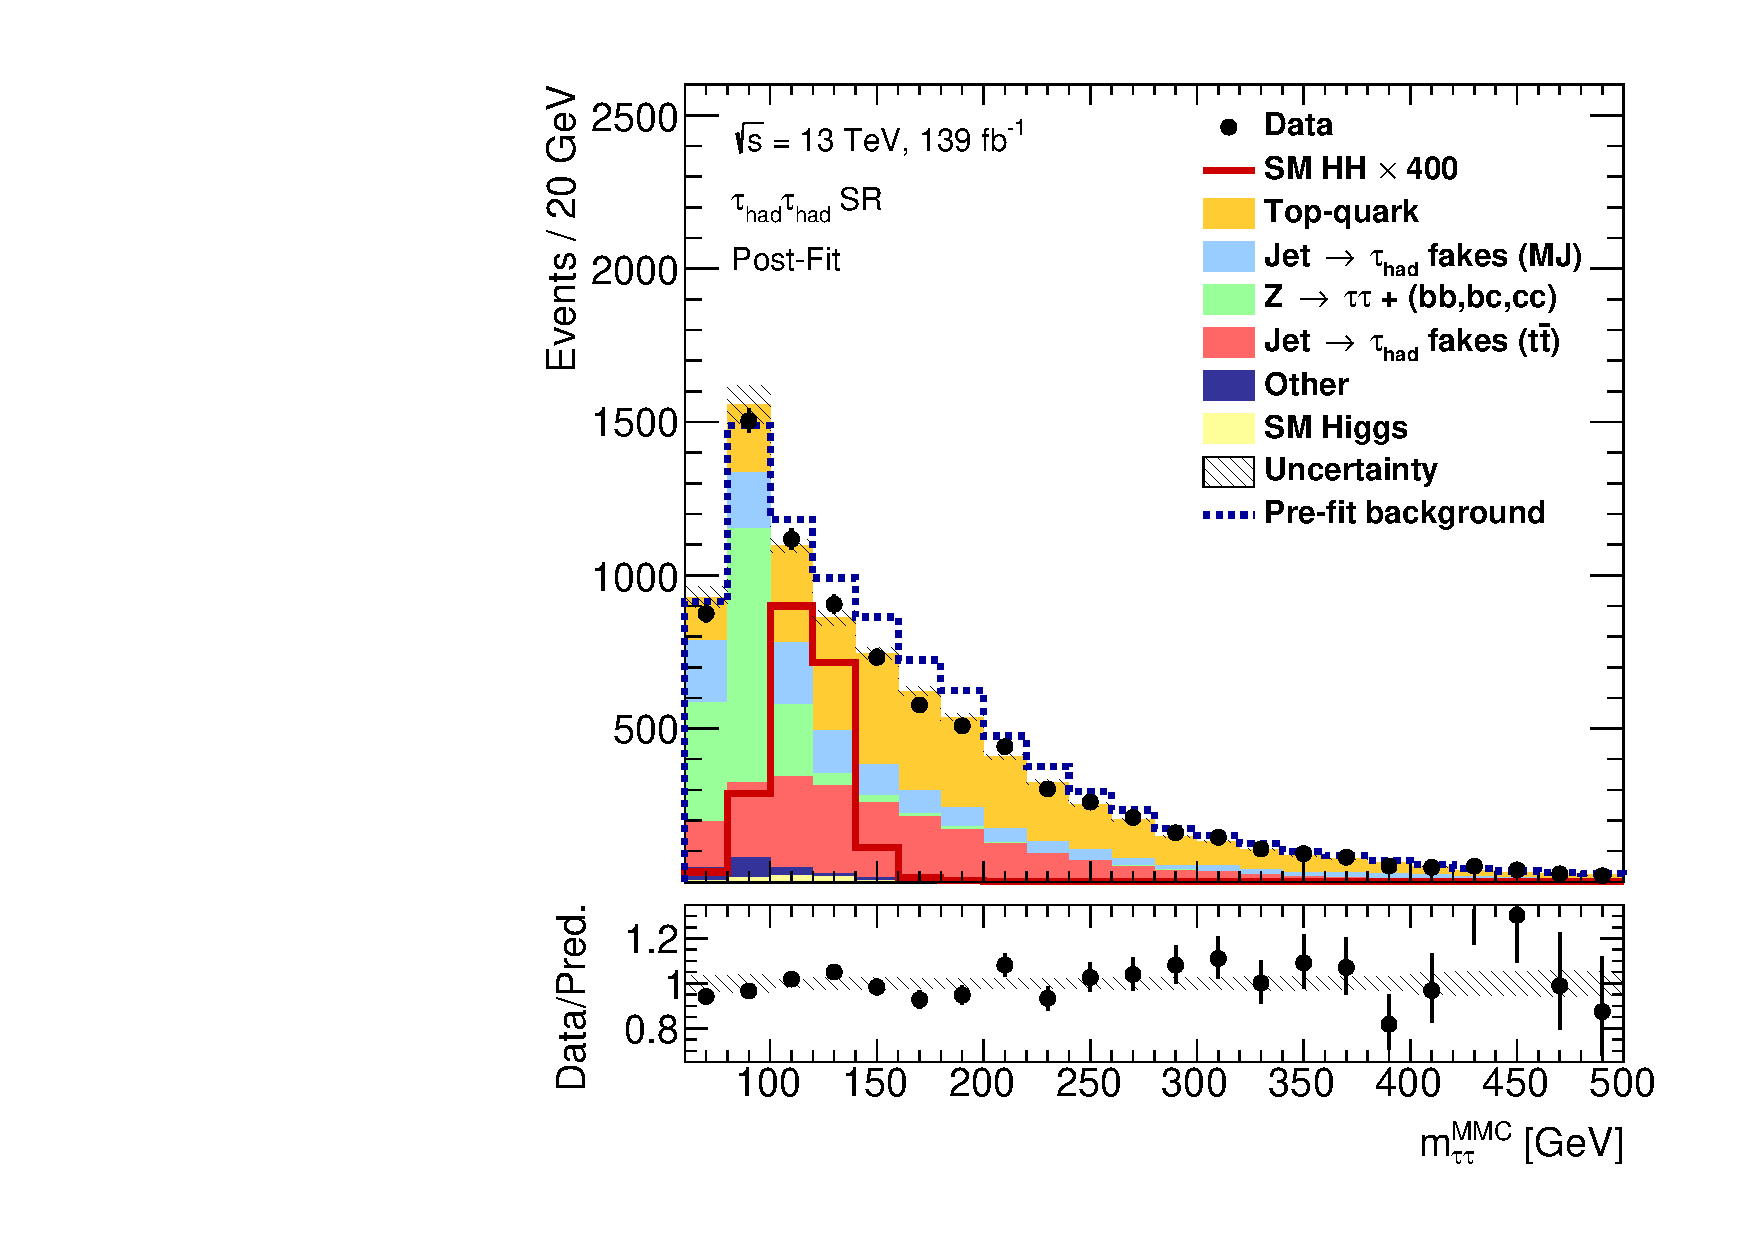
\includegraphics[width=\textwidth]{results_nonres/postfit_mvainputs/Region_BMin0_incJet1_distmMMC_J2_Y2015_DLLOS_T2_SpcTauHH_L0_GlobalFit_conditionnal_mu0}
  \end{subfigure}\hfill%
  \begin{subfigure}{0.46\textwidth}
    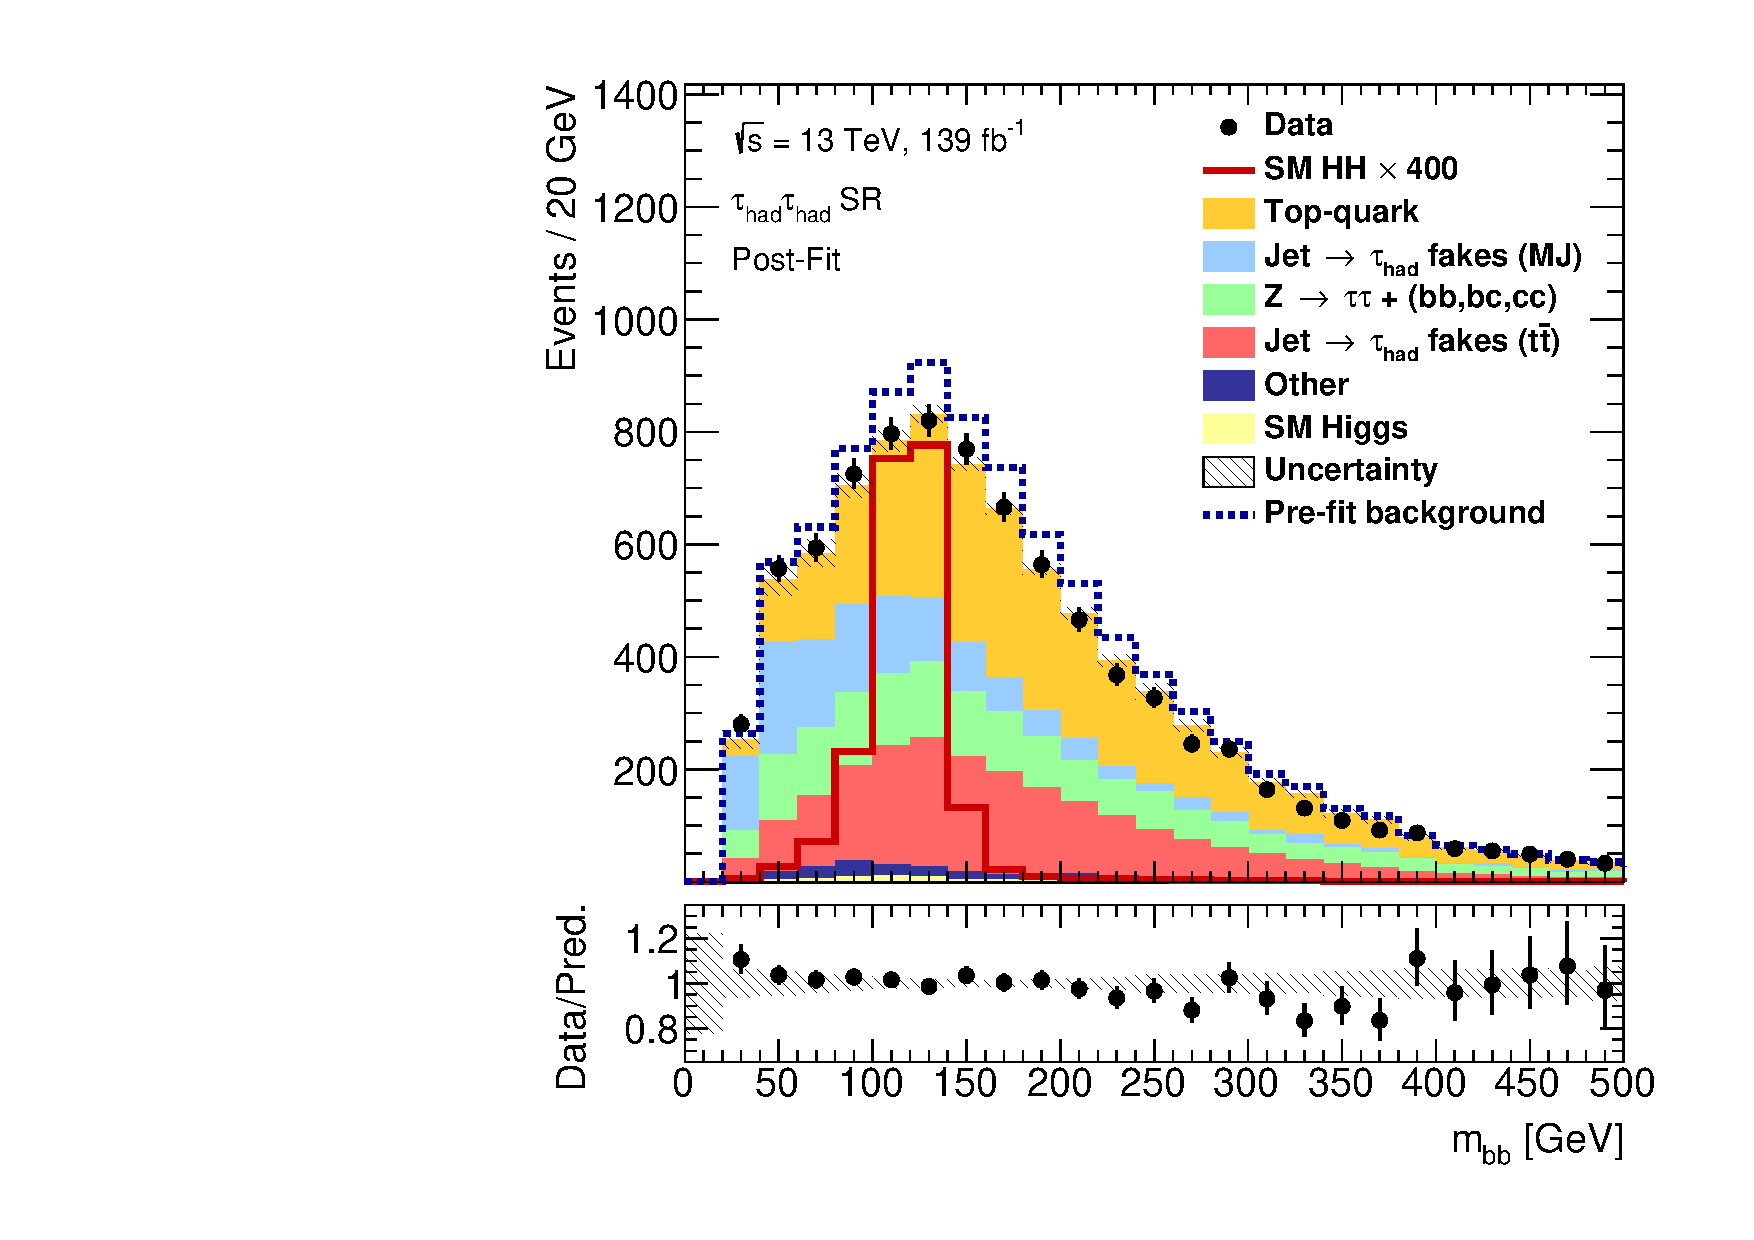
\includegraphics[width=\textwidth]{results_nonres/postfit_mvainputs/Region_BMin0_incJet1_distmBB_J2_Y2015_DLLOS_T2_SpcTauHH_L0_GlobalFit_conditionnal_mu0}
  \end{subfigure}

  \begin{subfigure}{0.46\textwidth}
    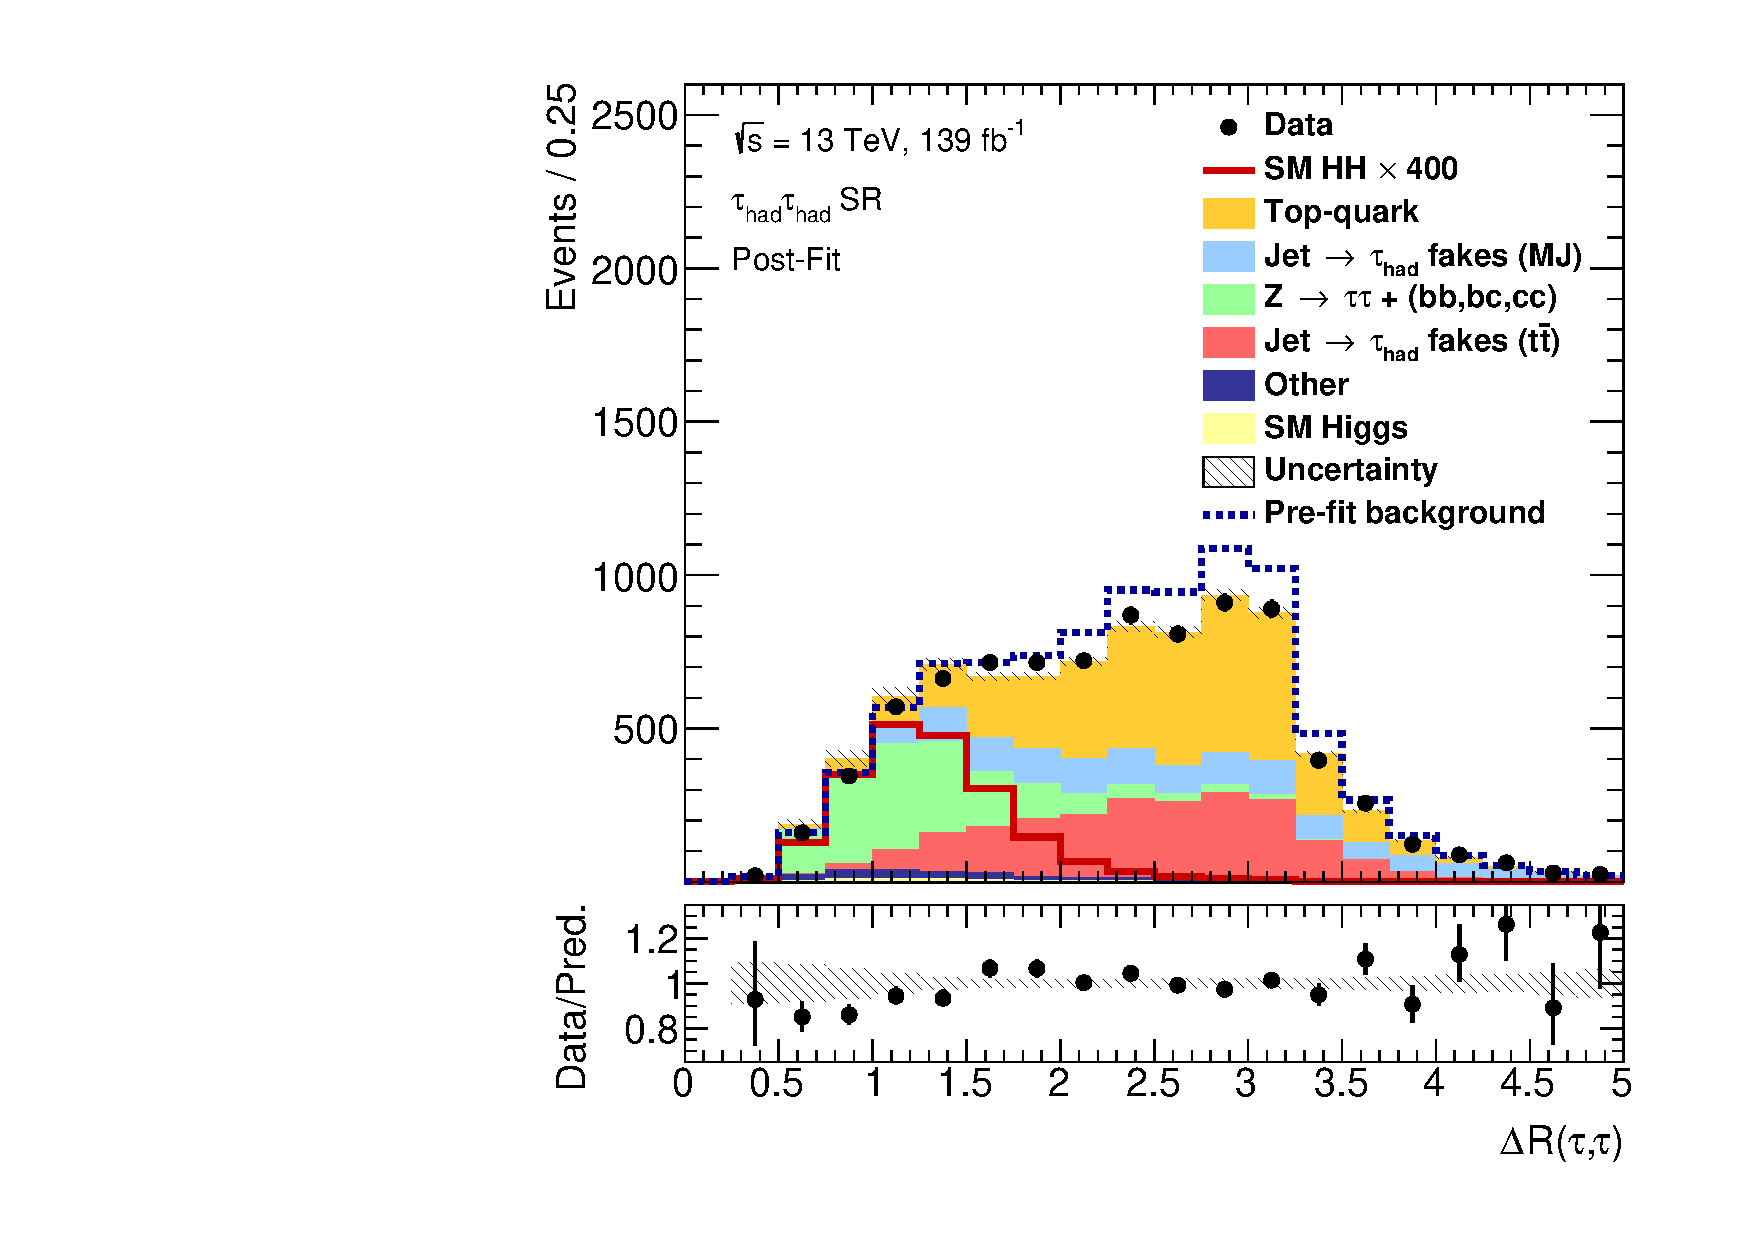
\includegraphics[width=\textwidth]{results_nonres/postfit_mvainputs/Region_BMin0_incJet1_distdRTauTau_J2_Y2015_DLLOS_T2_SpcTauHH_L0_GlobalFit_conditionnal_mu0_fontembed}
  \end{subfigure}\hfill%
  \begin{subfigure}{0.46\textwidth}
    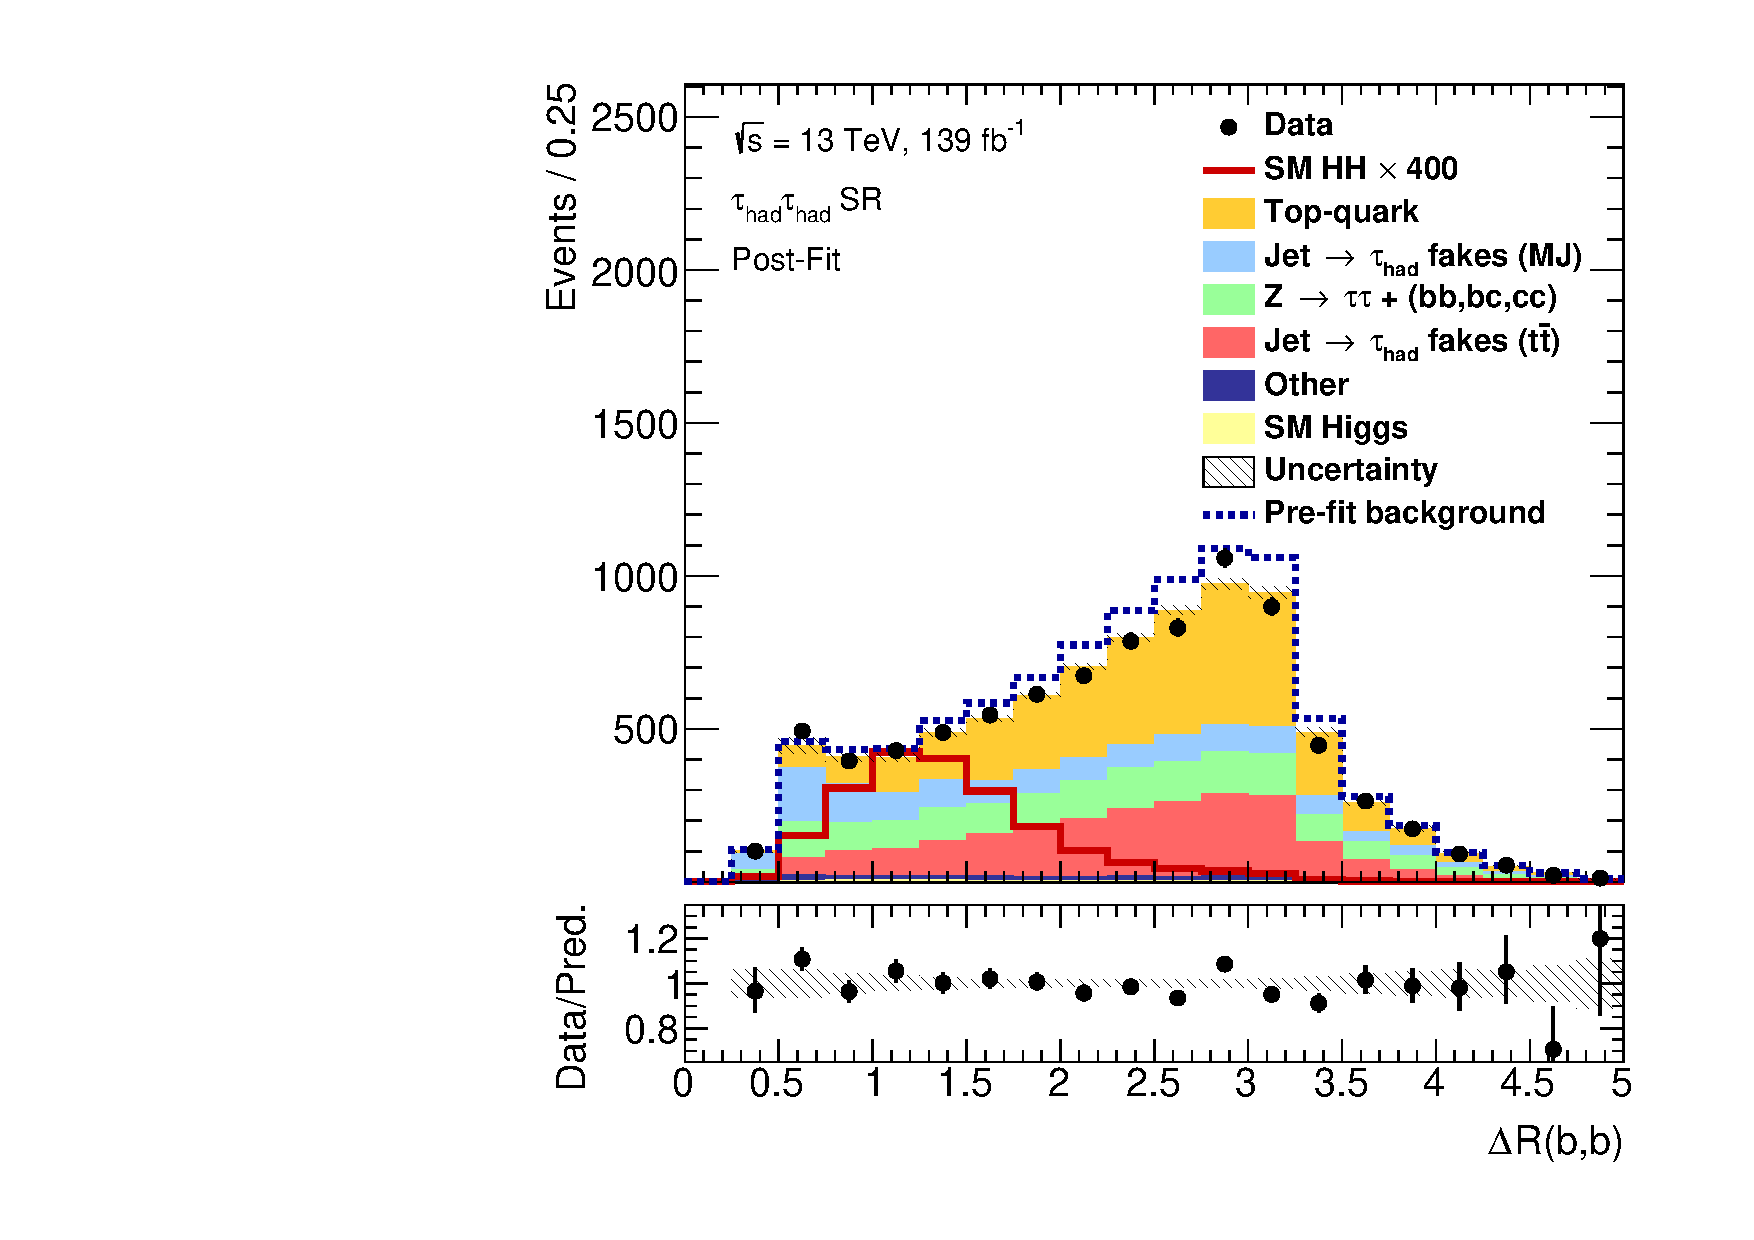
\includegraphics[width=\textwidth]{results_nonres/postfit_mvainputs/Region_BMin0_incJet1_distdRBB_J2_Y2015_DLLOS_T2_SpcTauHH_L0_GlobalFit_conditionnal_mu0_fontembed}
  \end{subfigure}

  \begin{subfigure}{0.46\textwidth}
    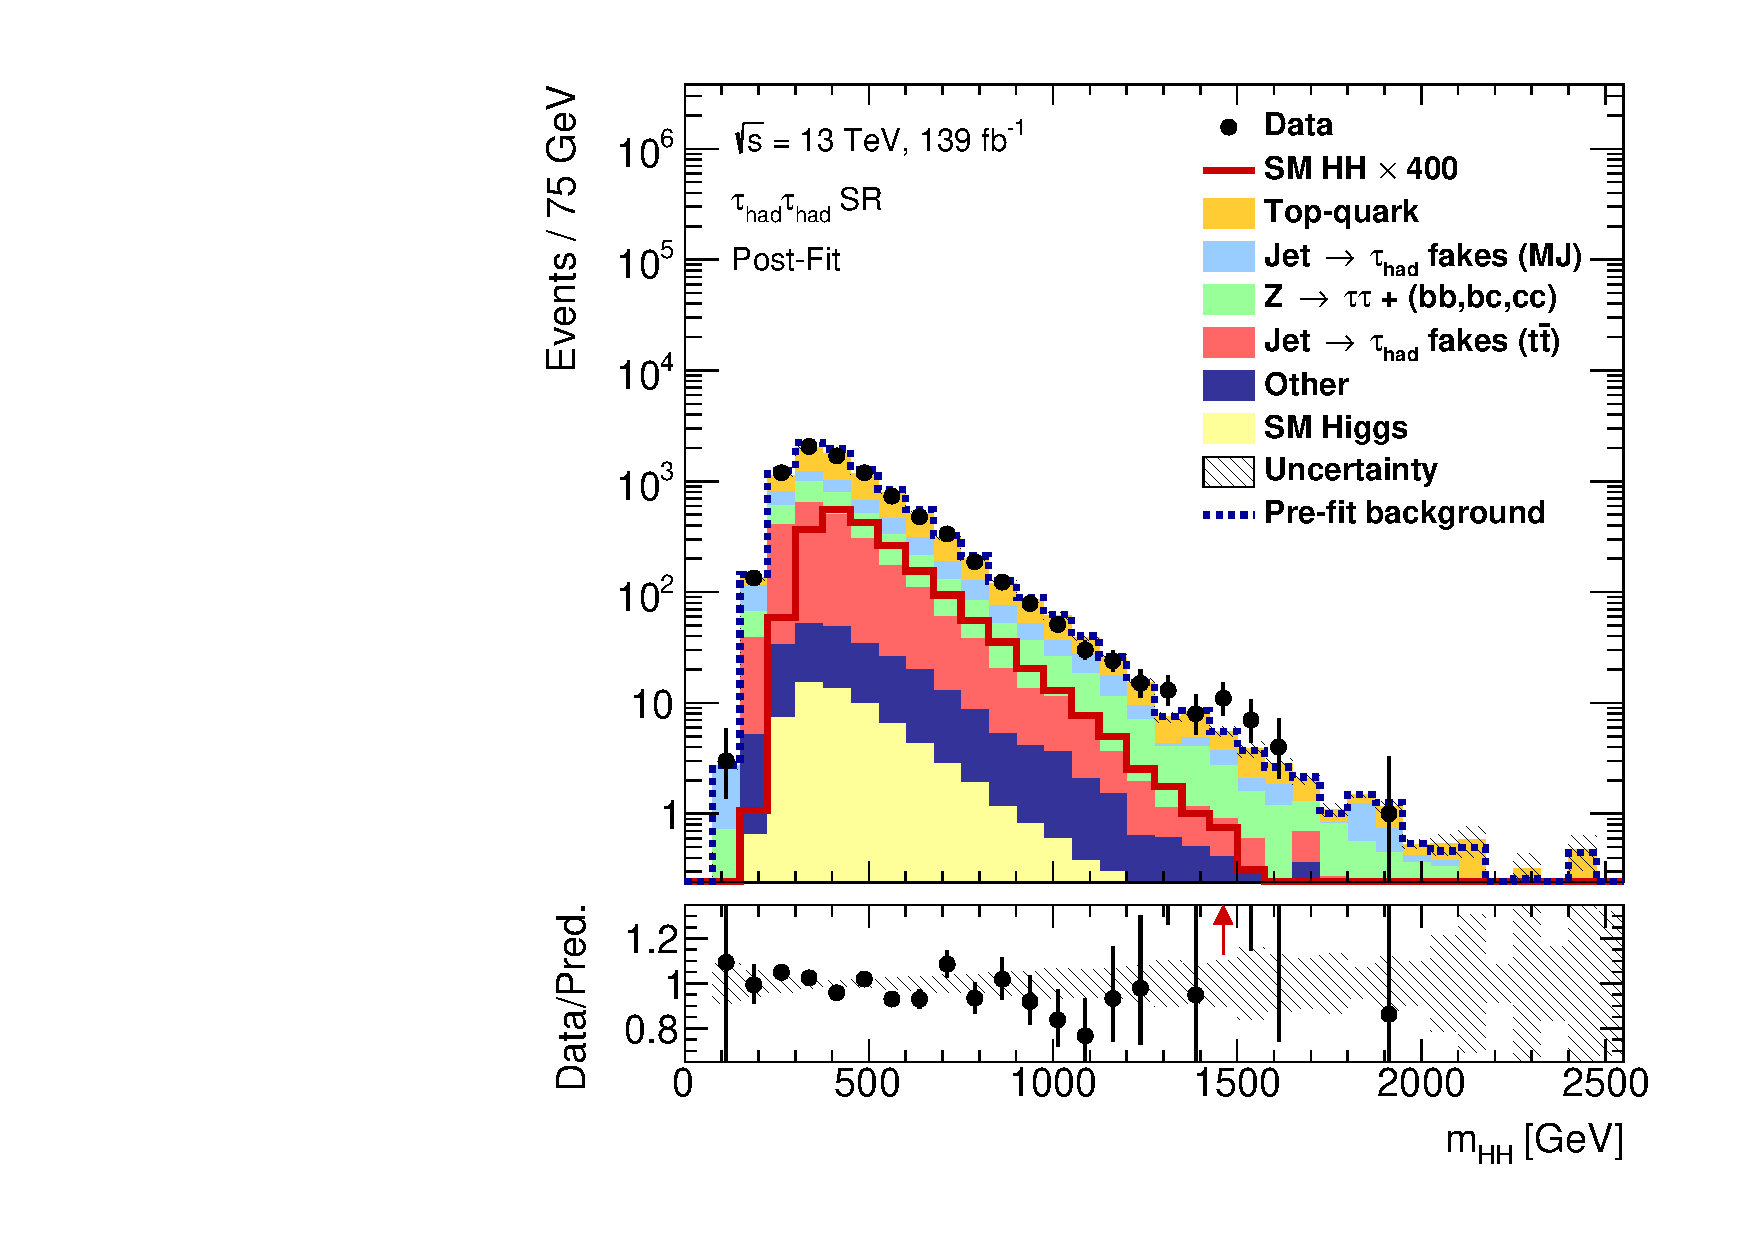
\includegraphics[width=\textwidth]{results_nonres/postfit_mvainputs/Region_BMin0_incJet1_distmHH_J2_Y2015_DLLOS_T2_SpcTauHH_L0_GlobalFit_conditionnal_mu0log}
  \end{subfigure}

  \caption[Distributions of the BDT input variables in the \hadhad SR after the
  background-only fit.]{Distributions of the BDT input variables in the \hadhad
    SR after the fit of the background-only model to observed data in all
    regions. The expected SM~\HH signal is overlayed with a normalisation
    corresponding to $\mu = 400$.}%
  \label{fig:postfit_mva_inputs}
\end{figure}

% q0 (obs): 0.357911
% sig (obs): 0.598257
% pval (obs): 0.274834

% SM (Asimov mu = 1)
% Median significance: 0.667530
% Median pValue: 0.252217
A comparison of the background-only and signal-plus-background hypothesis is
performed using a test for the discovery of a positive signal
(cf.~\Cref{sec:hypotesting}). This test yields an observed $p$-value of
\SI{27}{\percent}; thus, the background-only hypothesis cannot be rejected.
% (expected $p_0$-value of \SI{25.2}{\percent} from the $\mu = 1$ Asimov
% dataset)
Moreover, the signal strength obtained from the unconditional fit is
$\hat{\mu} = 0.9\,^{\hspace{0.25pt}+\hspace{0.25pt}1.8}_{-1.5}$ for the
combination of all channels, which is compatible with non-resonant \HH
production predicted by the SM but also with its absence.\footnote{The best-fit
  signal strength of the combination of \hadhad channel and \ZHF~CR
  is~$\hat{\mu} = 0.7\,^{\hspace{0.25pt}+\hspace{0.25pt}1.9}_{-1.6}$ and for the
  combination of the \lephad channels and
  \ZHF~CR~$\hat{\mu} = 1.9\,^{\hspace{0.25pt}+\hspace{0.25pt}3.7}_{-3.2}$.}

The dominant uncertainties affecting the measurement of the SM~\HH signal
strength are summarised in~\Cref{tab:breakdown_nonres} for the combination of
all channels. The measurement is mainly limited by the statistical uncertainty
originating from the small number of events observed at high values of the MVA
discriminants, which explains about $\frac{2}{3}$ of the variance on
\muhat. Systematic uncertainties play a lesser role, explaining about
$\frac{1}{3}$ of the variance on \muhat. The largest source of systematic
uncertainty are due to uncertainties on the modelling of backgrounds and the
statistical precision of the background estimate.

\begin{table}[htbp]
  \centering

  \caption[Breakdown of the variance of \muhat by uncertainty category for the
  SM~\HH search.]{Breakdown of the variance of \muhat by uncertainty category
    for the unconditional fit to observed data in all regions. The fraction of
    the variance on $\hat{\mu}$ from a category is approximated using
    $(\Delta\hat{\mu}^2_{\text{tot}} - \Delta\hat{\mu}^2_{\text{w/o cat}}) /
    \Delta \hat{\mu}^2_{\text{tot}}$, where $\Delta\hat{\mu}^2_{\text{tot}}$ is
    the estimate of the total variance of \muhat and
    $\Delta\hat{\mu}^2_{\text{w/o cat}}$ its variance after fixing the NPs of a
    given category to their best-fit values. The variance of \muhat from data
    statistical uncertainties is determined from the model with all NPs fixed to
    their best-fit values. The fractions of subcategories do not necessarily sum
    to the fraction of the parent category due to correlations between NPs.}%
  \label{tab:breakdown_nonres}

  % Estimated on non-resonant mu workspace
%
% Fractional impact of nuisance parameter sets, quadratically substracted from total.
% DataStat                     : + 0.649570732823647 / - 0.666811562391472 +- 0.657514352093487
% FullSyst                     : + 0.350429267176353 / - 0.333188437608528 +- 0.34240352840741
% All normalizations           : + 0.00256462411687674 / - 0.000629420848733356 +- 0.00150751388445714
% All but normalizations       : + 0.349881073822931 / - 0.332721677350132 +- 0.341893417327329
% Jets MET                     : + 0.00611881491094716 / - 0.00531445193052364 +- 0.00573985723146677
% BTag                         : + 0.00273018206308313 / - 0.00251352205815197 +- 0.00262889128845151
% Electron Muon                : + 0.00147658980045641 / - 0.000764053590433247 +- 0.0011182187740484
% Tau                          : + 0.00557804691013822 / - 0.00126289813038191 +- 0.0032018485963158
% Pileup reweighting           : + 6.42848069842953e-05 / - 0.000110024034672235 +- 8.39149975446109e-05
% Fake estimation              : + 0.0073527804179163 / - 0.00585172181539581 +- 0.00663745433087985
% Luminosity                   : + 0.00149085233805505 / - 0.000167571652278191 +- 0.000715242667614943
% Top Modelling                : + 0.0604793187664376 / - 0.0562464434201449 +- 0.0585030684775916
% Ztautau+HF Modelling         : + 0.00845814093617601 / - 0.0102153499042302 +- 0.00925002791617588
% Single Higgs Modelling       : + 0.0617151711880666 / - 0.107540079213718 +- 0.0813319338742543
% Signal Modelling             : + 0.0941027334483326 / - 0.00501948112092907 +- 0.0390780989113785
% Other backgrounds            : + 0.000775646139682544 / - 0.00124168478503861 +- 0.000977564478036541
% MC stat                      : + 0.0590496581302566 / - 0.10019920077973 +- 0.0767316565018313
% Instrumental (Chris)         : + 0.0168480040103595 / - 0.0109929390836323 +- 0.0139860056583981
% Signal modelling (Chris)     : + 0.0941027334483326 / - 0.00501948112092907 +- 0.0390780989113785
% Background modelling (Chris) : + 0.162826849351099 / - 0.208956381988409 +- 0.183441723017023

\begin{tabular}{lS[table-format=2.0, table-space-text-pre=\textless]}
  \toprule
         & {Explained fraction} \\
  Source & {of variance on $\hat{\mu}$} \\
  \midrule
  \textbf{Data statistical uncertainty} & 66\,\si{\percent} \\  %81\,\si{\percent} \\
  \textbf{Systematic uncertainties} & 34\,\si{\percent} \\  %58\,\si{\percent} \\
  \hspace{0.8em} Instrumental uncertainties & 1\,\si{\percent} \\  %11\,\si{\percent} \\
  \hspace{0.8em} Signal modelling uncertainties & 4\,\si{\percent} \\
  \hspace{0.8em} Background statistical uncertainties & 8\,\si{\percent} \\  %28\,\si{\percent} \\
  \hspace{0.8em} Background modelling uncertainties & 18\,\si{\percent} \\  %42\,\si{\percent} \\
  \midrule
  \hspace{1.6em} -- \hspace{0.2em} Top-quark (incl.\ free normalisation) & 6\,\si{\percent} \\
  \hspace{1.6em} -- \hspace{0.2em} \ZHF (incl.\ free normalisation) & 1\,\si{\percent} \\
  \hspace{1.6em} -- \hspace{0.2em} SM Higgs boson & 8\,\si{\percent} \\
  \hspace{1.6em} -- \hspace{0.2em} Fake-\tauhadvis & {\textless } 1\,\si{\percent} \\
  \hspace{1.6em} -- \hspace{0.2em} Other & {\textless } 1\,\si{\percent} \\
  \bottomrule
\end{tabular}

% {$( \Delta \mu_{\text{tot}}^2 - \Delta \mu_{\text{categ.}}^2  ) / \Delta \mu_{\text{tot}}^2$} \\

%%% Local Variables:
%%% mode: latex
%%% TeX-master: "../phd_thesis"
%%% End:

\end{table}

The effect of uncertainties on \muhat is examined on the level of individual NPs
in~\Cref{fig:nonres_np_rankings}, separately for the \hadhad and \lephad
channels as well as their combination. A ranking of NPs with the largest impact
on the estimated signal strength is shown in the figure, including the MLE of
the NPs and their \SI{68}{\percent} confidence intervals. Generally, the NPs are
compatible with their pre-fit values. For few NPs the fit provides more
stringent constraints than suggested by their prior measurement, which is
consistent with results from fits to Asimov dataset.

The largest constraint observed in the \hadhad channel is on the NP related to
the \ZHF acceptance uncertainty determined by an MC-to-MC comparison of
\SHERPA~(NLO) and \MGPY~(LO). This uncertainty is conservative since it compares
the nominal matrix element generator at NLO with a lower order
prediction. Therefore, the associated NP is expected to be constrained in the
fit. In the \lephad channel, large constraints are observed on the NP associated
with the uncertainty on \rqcd and the \ttbar acceptance uncertainty from the
comparison of parton shower programs. The uncertainty on \rqcd is derived to be
conservative, varying \rqcd between 0 and \SI{100}{\percent}, explaining the
large constraints on this parameter.
% the assumed fraction of \faketauhadvis originating from multi-jet processes in
% the anti-\tauhadvis CR between 0 and \SI{100}{\percent}, explaining the large
% constraints on this parameter.
The constraints on the \ttbar acceptance uncertainty based on the parton shower
comparison originates in the \lephad SLT channel. Since the constraint is large,
this uncertainty source is decorrelated between channels to prevent
underestimating the acceptance uncertainty in other channels.

\begin{sidewaysfigure}[p]
  \centering

  \begin{subfigure}{0.328\textwidth}
    \centering
    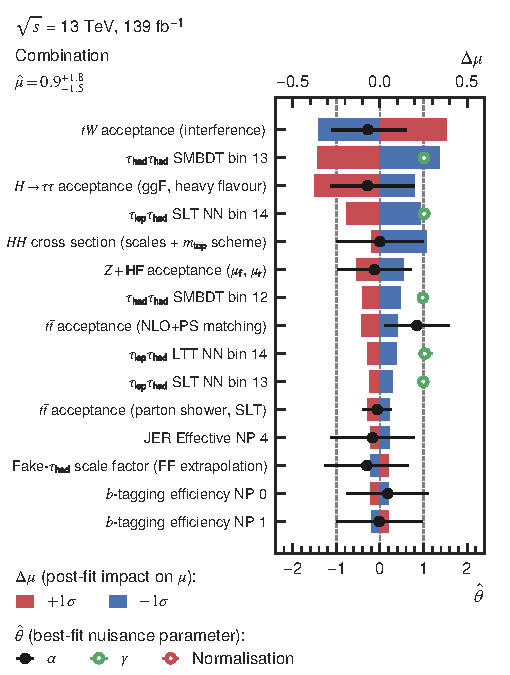
\includegraphics[width=\textwidth, trim=0.2em 0 1em 0, clip]{results_nonres/rankings/ranking_nonres_combined}
    \subcaption{Combination of all channels}
  \end{subfigure}\hfill%
  \begin{subfigure}{0.328\textwidth}
    \centering
    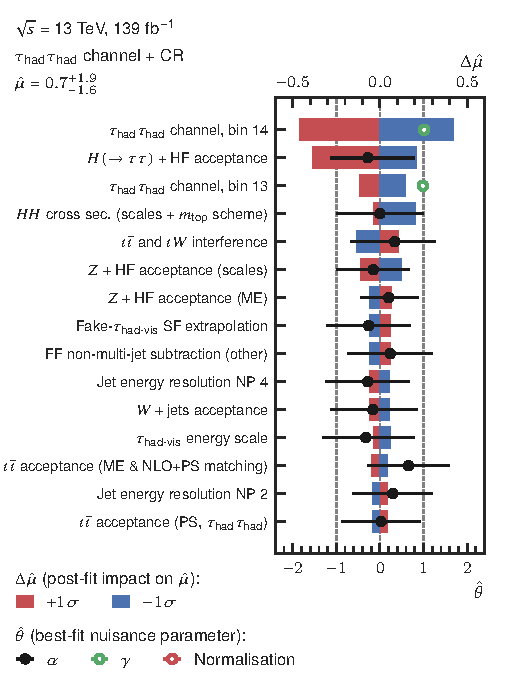
\includegraphics[width=\textwidth, trim=0.2em 0 1em 0, clip]{results_nonres/rankings/ranking_nonres_hadhad}
    \subcaption{\hadhad channel and \ZHF CR}%
    \label{fig:nonres_np_ranking_hadhad}
  \end{subfigure}\hfill%
  \begin{subfigure}{0.328\textwidth}
    \centering
    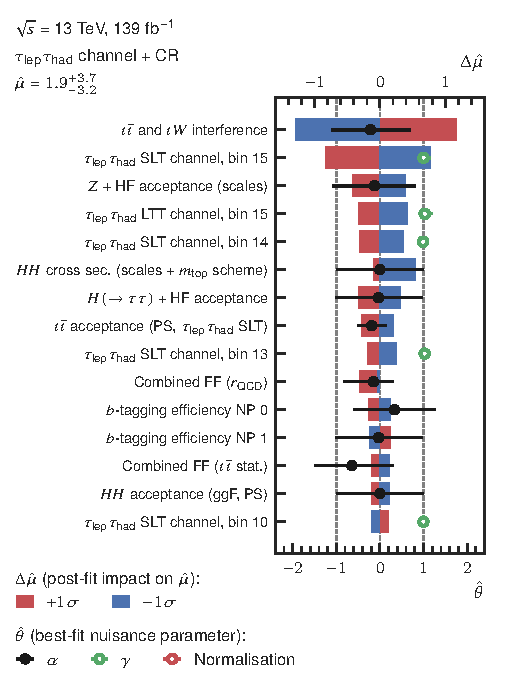
\includegraphics[width=\textwidth, trim=0.2em 0 1em 0, clip]{results_nonres/rankings/ranking_nonres_lephad}
    \subcaption{\lephad channels and \ZHF CR}
  \end{subfigure}

  \caption[Post-fit pulls and rankings of NPs for the fit of all regions, the
  \hadhad SR and \ZHF~CR, and the \lephad SRs and \ZHF~CR.]{Ranking of NPs based
    on the post-fit impact on \muhat as measured by the change in the estimated
    signal strength~$\Delta \hat{\mu}$ when performing the fit after fixing a
    given NP to $\hat{\theta} \pm \Delta \hat{\theta}$, where $\hat{\theta}$ is
    the MLE and $\Delta \hat{\theta}$ the post-fit uncertainty on the NP. The
    impact on \muhat is shown on the top axis and the NPs are given in
    descending order of the mean~$|\Delta \hat{\mu}|$. The bottom axis shows the
    MLE of the NPs and the post-fit uncertainty, with marker colours indicating
    the type of NP:~NPs with Gaussian constraints~($\alpha$, black), NPs with
    Poisson constraints from the Barlow--Beeston method~($\gamma$, green), and
    normalisation factors~(red). The rankings are obtained from fits of the
    signal-plus-background model to observed data in all regions (a), in the
    \hadhad SR and \ZHF~CR (b), and in the \lephad SRs and \ZHF~CR (c).}%
  \label{fig:nonres_np_rankings}
\end{sidewaysfigure}

Although the analysis is mostly limited by the size of the recorded
\pp~collision dataset, a few of the leading sources of uncertainty are discussed
in the following:
\begin{itemize}

\item Statistical uncertainties on the expected background rates in high MVA
  score bins are among the uncertainties with the largest impact on the analysis
  sensitivity. The MC simulations used for background estimation only populate
  the high MVA score regions sparsely, resulting in large statistical
  uncertainties. In addition, the \faketauhadvis background estimation in the
  \hadhad~channel requires a large subtraction of non-multi-jet events that
  further reduces the statistical precision of the background rate
  predictions. As a result, the associated uncertainties have non-negligible
  effect on the sensitivity of the analysis.

  % Statistical uncertainties on the background prediction have a large impact
  % when comparing to other systematic uncertainties. These uncertainties arise
  % from the finite number of simulated events used for the background predictions
  % and the number of CR events used to perform the data-driven \faketauhadvis
  % background estimates.

  % The distinct features of Higgs boson pair production in the SM allow to
  % separate the targeted signal well from most background processes when
  % employing multivariate techniques. Therefore, simulation-based background
  % predictions, while generally produced with integrated luminosities exceeding
  % that of the collected data,\footnote{The data statistical uncertainties, not
  % the statistical precision of the background prediction, are the primary
  % limitation for the signal extraction as can be seen
  % in~\Cref{tab:breakdown_nonres}.} do not populate the region of high MVA
  % scores densely, leading to non-negligible statistical uncertainties on the
  % background predictions in the most signal-like bins.

  % Additionally, the data-driven estimate of the multi-jet background in the
  % \hadhad channel includes large subtractions of non-multi-jet events in the
  % CR, further degrading the statistical precision of the background
  % estimate. As a result, in the \hadhad-only fit the associated NP has the
  % largest impact of any single NP on the extracted signal strength (cf.\
  % $\gamma$ NP for SMBDT bin 13 in~\Cref{fig:nonres_np_ranking_hadhad}).

\item The $tW$ acceptance uncertainty targeting the $tW$ and \ttbar interference
  is the systematic uncertainty with the largest impact on $\mu$ in the \lephad
  channels and the combination. The large impact originates from the \lephad SLT
  channel, where the uncertainty can reach up to \SI{80}{\percent} at high NN
  score. Moreover, $tW$ production makes up half of the top-quark background at
  high NN score in the \lephad SLT channel. This uncertainty is less relevant in
  the \hadhad and \lephad LTT channels due to smaller fractions of $tW$ events
  in the most signal-like bins of the MVA discriminants.

\item The uncertainty of \SI{100}{\percent} on the acceptance of
  $gg \to H \to \tautau$ production in association with quarks of heavy flavour
  has a large impact on the fitted $\mu$. The most signal-like bins of the BDT
  discriminant in the \hadhad channel select a considerable amount of single
  Higgs boson events (cf.~\Cref{tab:postfit_yields_smhh_signallike}). About a
  fourth of these events are expected to be from $H \to \tautau$ production via
  \ggF, which are subject to the heavy flavour uncertainty. As a result, this
  uncertainty is among the leading uncertainties affecting the background
  prediction in the most signal-like bins.

\end{itemize}
% The effect of uncertainties is similar to the previous Run~2
% analysis~\cite{HIGG-2016-16-witherratum} using a partial dataset of \pp
% collisions at $\sqrt{s} = \SI{13}{\TeV}$ with \SI{36.1}{\per\femto\barn}
% integrated luminosity.
%
% \todo[inline]{Discussion: Impact of data statistical uncertainties is about
% the same -> Speaks for improvements in CP and the analysis. Instrumental
% decreased in full Run~2. Huge improvements in calibration measurements.}

Given the absence of a statistically significant signal, upper limits are set on
the SM~\HH signal strength and cross section using the \CLs method at
\SI{95}{\percent}~CL. \Cref{tab:limits_non_resonant} summarises the exclusion
limits separately for the \lephad channels, the \hadhad channel, and their
combination. The observed (expected) upper limit on the signal strength is
\num{4.7} (\num{3.9}) for the combination of all channels. The upper limits are
largely driven by the high sensitivity of the \hadhad channel to SM~\HH
production, yielding observed (expected) upper limits on $\mu$ of \num{5.0}
(\num{4.4}). Further discussion of these results is given
in~\Cref{sec:result_discussion}.

\begin{table}[htbp]
  \centering

  \caption[Upper limits on the SM~\HH production cross section and signal
  strength at \SI{95}{\percent}~CL.]{Upper limits on the SM~\HH production cross
    section via \ggF and VBF, \xsecggfvbf, and the SM~\HH signal strength,
    $\mu$, at \SI{95}{\percent}~CL.  The expected limits are obtained under the
    assumption of the background-only hypothesis. The table is adapted from
    Ref.~\cite{HDBS-2018-40}.}%
  \label{tab:limits_non_resonant}

  % Workspaces: comb_2022_01_29
  % ==================
% Channel: combined
% Upper limit on mu:
%         Obs.     -2sigma     -1sigma        Exp.     +1sigma     +2sigma
%     4.700596    2.082483    2.795737    3.879976    5.399804    7.238819

% Upper limit on xsec [fb]:
%         Obs.     -2sigma     -1sigma        Exp.     +1sigma     +2sigma
%     136.6652     61.5679     82.6550    114.7102    159.6434    214.0133

% ==================
% ==================
% Channel: hadhad
% Upper limit on mu:
%         Obs.     -2sigma     -1sigma        Exp.     +1sigma     +2sigma
%     4.951880    2.371052    3.183142    4.417624    6.148054    8.241901

% Upper limit on xsec [fb]:
%         Obs.     -2sigma     -1sigma        Exp.     +1sigma     +2sigma
%     145.1928     70.4159     94.5334    131.1952    182.5858    244.7692

% ==================
% ==================
% Channel: lephad
% Upper limit on mu:
%         Obs.     -2sigma     -1sigma        Exp.     +1sigma     +2sigma
%     9.679448    4.205958    5.646506    7.836325   10.905898   14.620128

% Upper limit on xsec [fb]:
%         Obs.     -2sigma     -1sigma        Exp.     +1sigma     +2sigma
%     281.6663    124.3330    166.9173    231.6509    322.3910    432.1879

% ==================
\begin{tabular}{
  lc
  S[table-format=3.1, round-mode=figures, round-precision=2]
  S[table-format=3.1, round-mode=figures, round-precision=2]
  S[table-format=3.1, round-mode=figures, round-precision=2]
  S[table-format=3.1, round-mode=figures, round-precision=2]
  S[table-format=3.1, round-mode=figures, round-precision=2]
  S[table-format=3.1, round-mode=figures, round-precision=2]
  }
  \toprule
  && {Observed} & {$-2\sigma$} & {$-1\sigma$} & {Expected} & {$+1\sigma$} & {$+2\sigma$} \\
  \midrule
  \multirow{2}{*}{\lephad channel} & {$\xsecggfvbf \, / \, \si{\femto\barn}$} & 281.6663 & 124.3330 & 166.9173 & 231.6509 & 322.3910 & 432.1879 \\
                                   & {$\mu$} & 9.679448 & 4.205958 & 5.646506 & 7.836325 & 10.905898 & 14.620128 \\
  \midrule
  \multirow{2}{*}{\hadhad channel} & {$\xsecggfvbf \, / \, \si{\femto\barn}$} & 145.1928 & 70.4159 & 94.5334 & 131.1952 & 182.5858 & 244.7692 \\
                                   & {$\mu$} & 4.951880 & 2.371052 & 3.183142 & 4.417624 & 6.148054 & 8.241901 \\
  \midrule
  \multirow{2}{*}{Combination}     & {$\xsecggfvbf \, / \, \si{\femto\barn}$} & 136.6652 & 61.5679 & 82.6550 & 114.7102 & 159.6434 & 214.0133 \\
                                   & {$\mu$} & 4.700596 & 2.082483 & 2.795737 & 3.879976 & 5.399804 & 7.238819 \\
  \bottomrule
\end{tabular}

%%% Local Variables:
%%% mode: latex
%%% TeX-master: "../phd_thesis"
%%% End:

\end{table}


\subsection{Results of the Search for Resonant \HH Production}%
\label{sec:results_res}

The search for resonant \HH production uses the cross
section~$\sigma(\pp \to X \to \HH)$ as the POI. Otherwise, the statistical
interpretation proceeds in analogy to the SM~\HH case after replacing the BDT/NN
discriminants by PNN discriminants evaluated with mass parameters set to the \mX
of the signal hypothesis of interest.

The PNN discriminants in the \hadhad~SR are shown for four exemplary mass points
in~\Cref{fig:resonant_mva_postfit} after the background-only fit to observed
data in all regions. Moreover, \Cref{tab:yields_postfit_resonant} summarises the
expected number of events in a signal-like region of the PNN discriminant after
the fit. Figures of the PNN discriminants in the \lephad channels are summarised
in~\Cref{app:pnn_plots_lephad}. The background processes relevant to the search
vary with the \mX of the considered signal hypothesis. For low-mass resonances,
the dominant backgrounds are top-quark production and \faketauhadvis
backgrounds. These background processes become less important for larger \mX, at
which point the production of \Zjets becomes the dominant background.

\begin{figure}[htbp]
  \centering

  \begin{subfigure}{0.495\textwidth}
    \centering

    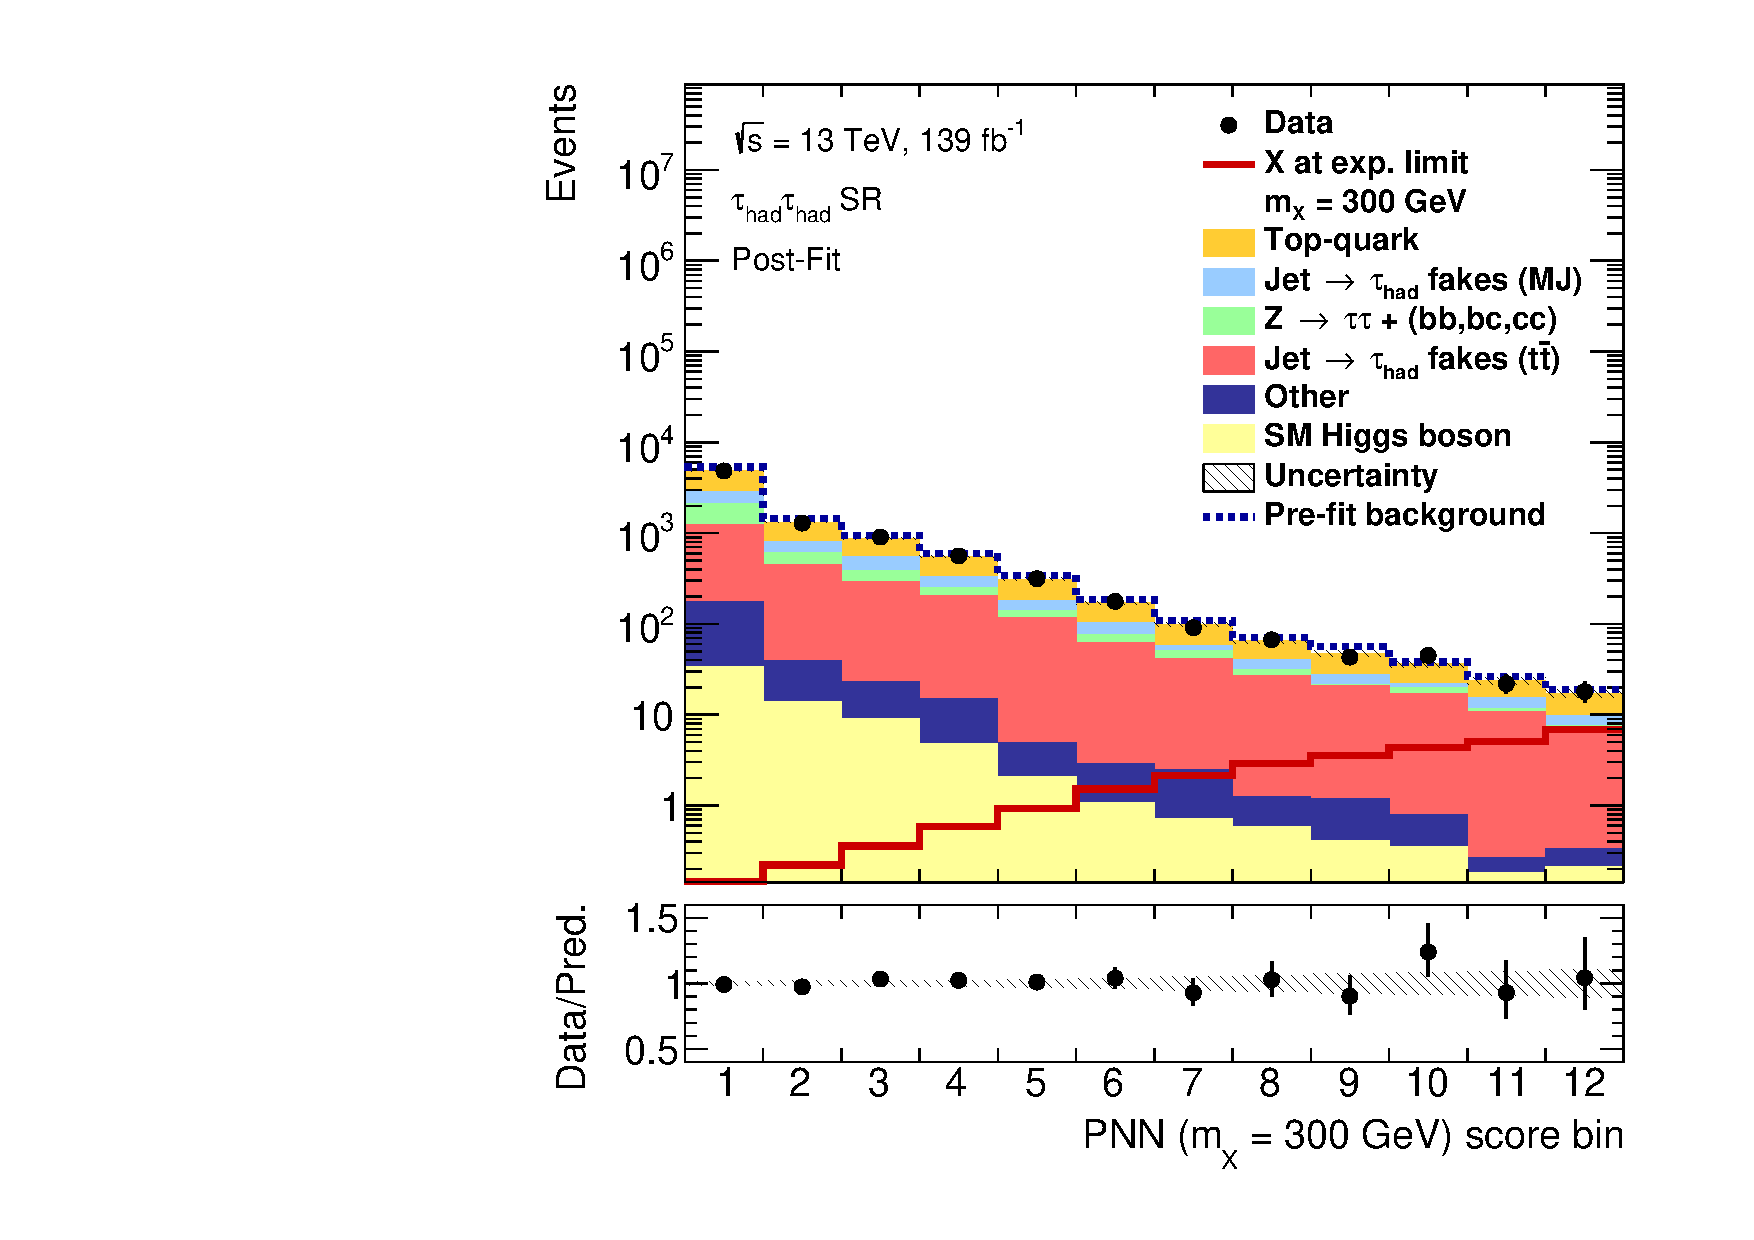
\includegraphics[width=\textwidth]{results_res/postfit/Region_BMin0_incJet1_distPNN300_J2_Y2015_DLLOS_T2_SpcTauHH_L0_GlobalFit_conditionnal_mu0log}
    \subcaption{$\mX = \SI{300}{\GeV}$}
  \end{subfigure}\hfill%
  \begin{subfigure}{0.495\textwidth}
    \centering

    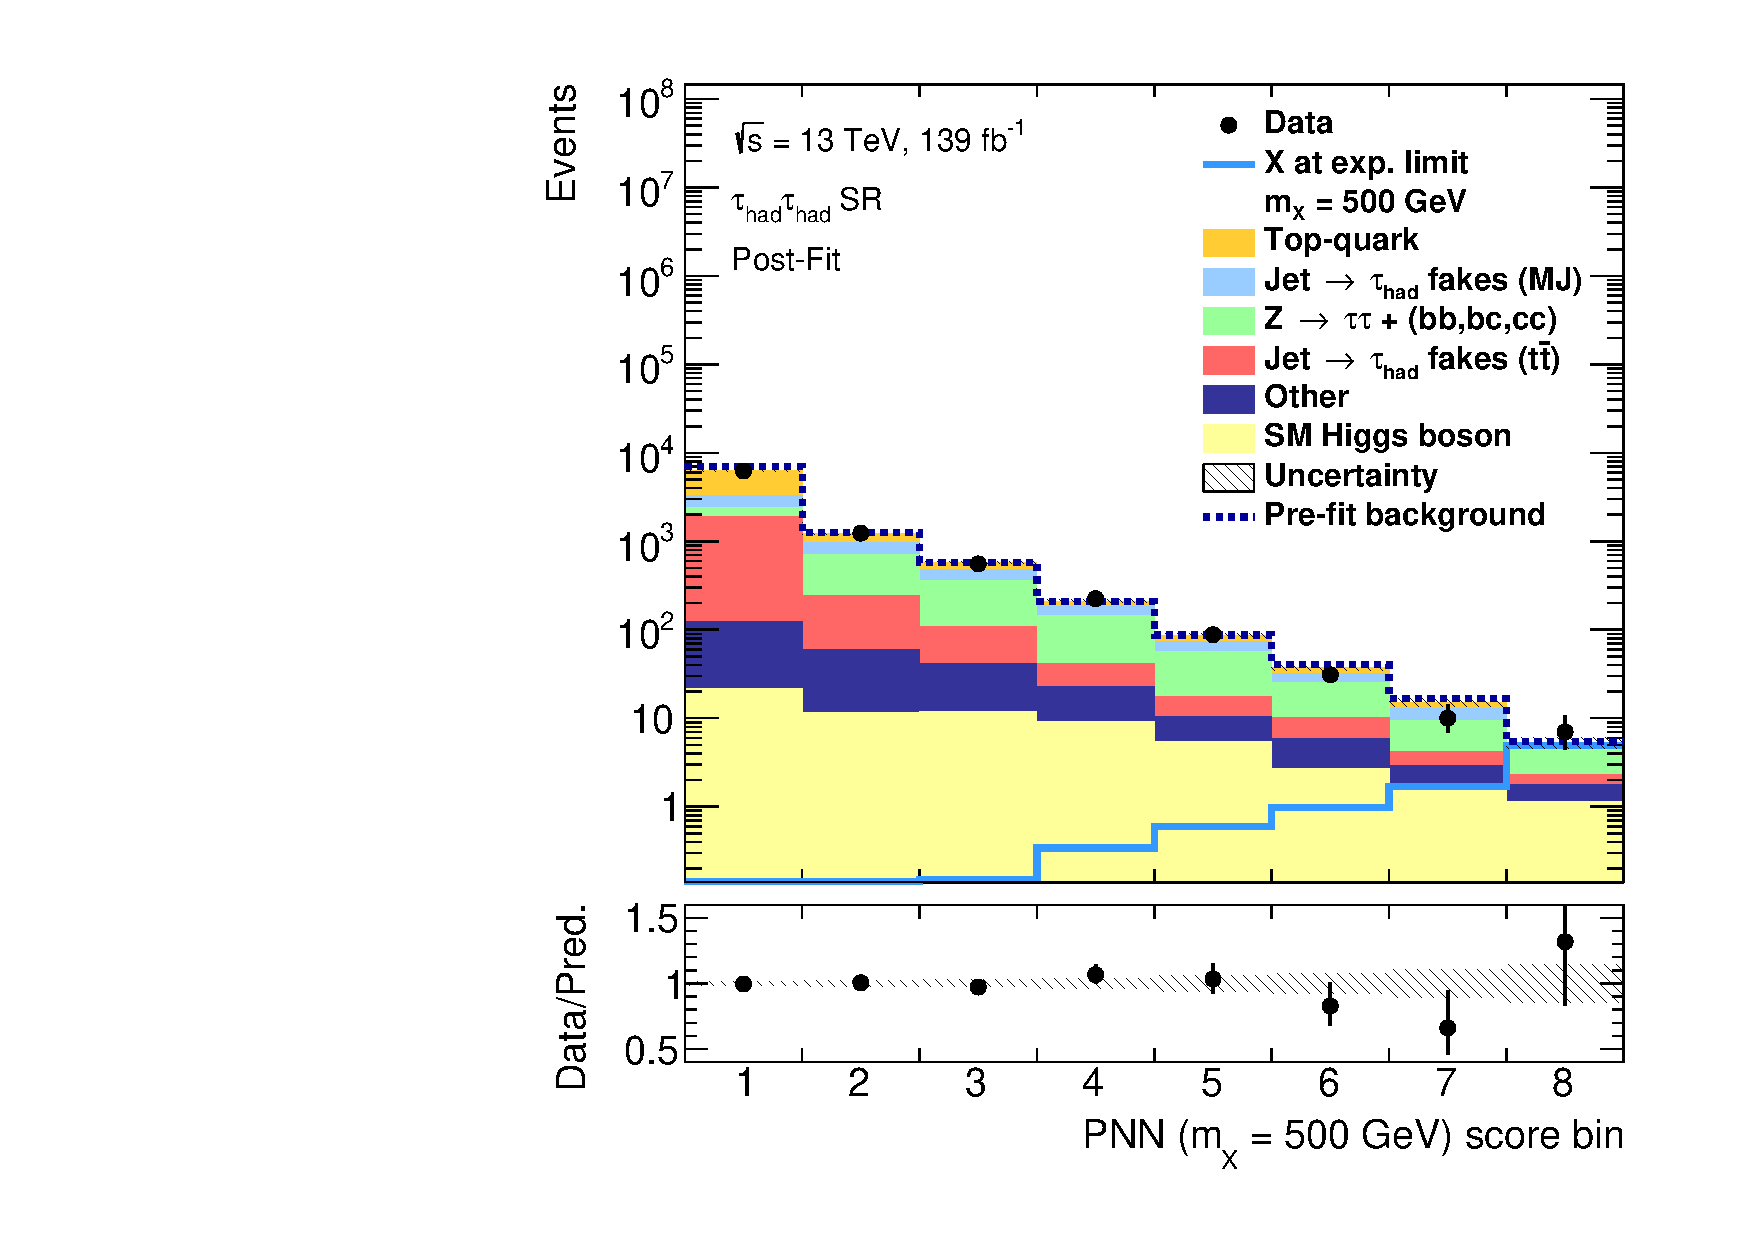
\includegraphics[width=\textwidth]{results_res/postfit/Region_BMin0_incJet1_distPNN500_J2_Y2015_DLLOS_T2_SpcTauHH_L0_GlobalFit_conditionnal_mu0log}
    \subcaption{$\mX = \SI{500}{\GeV}$}
  \end{subfigure}

  \begin{subfigure}{0.495\textwidth}
    \centering

    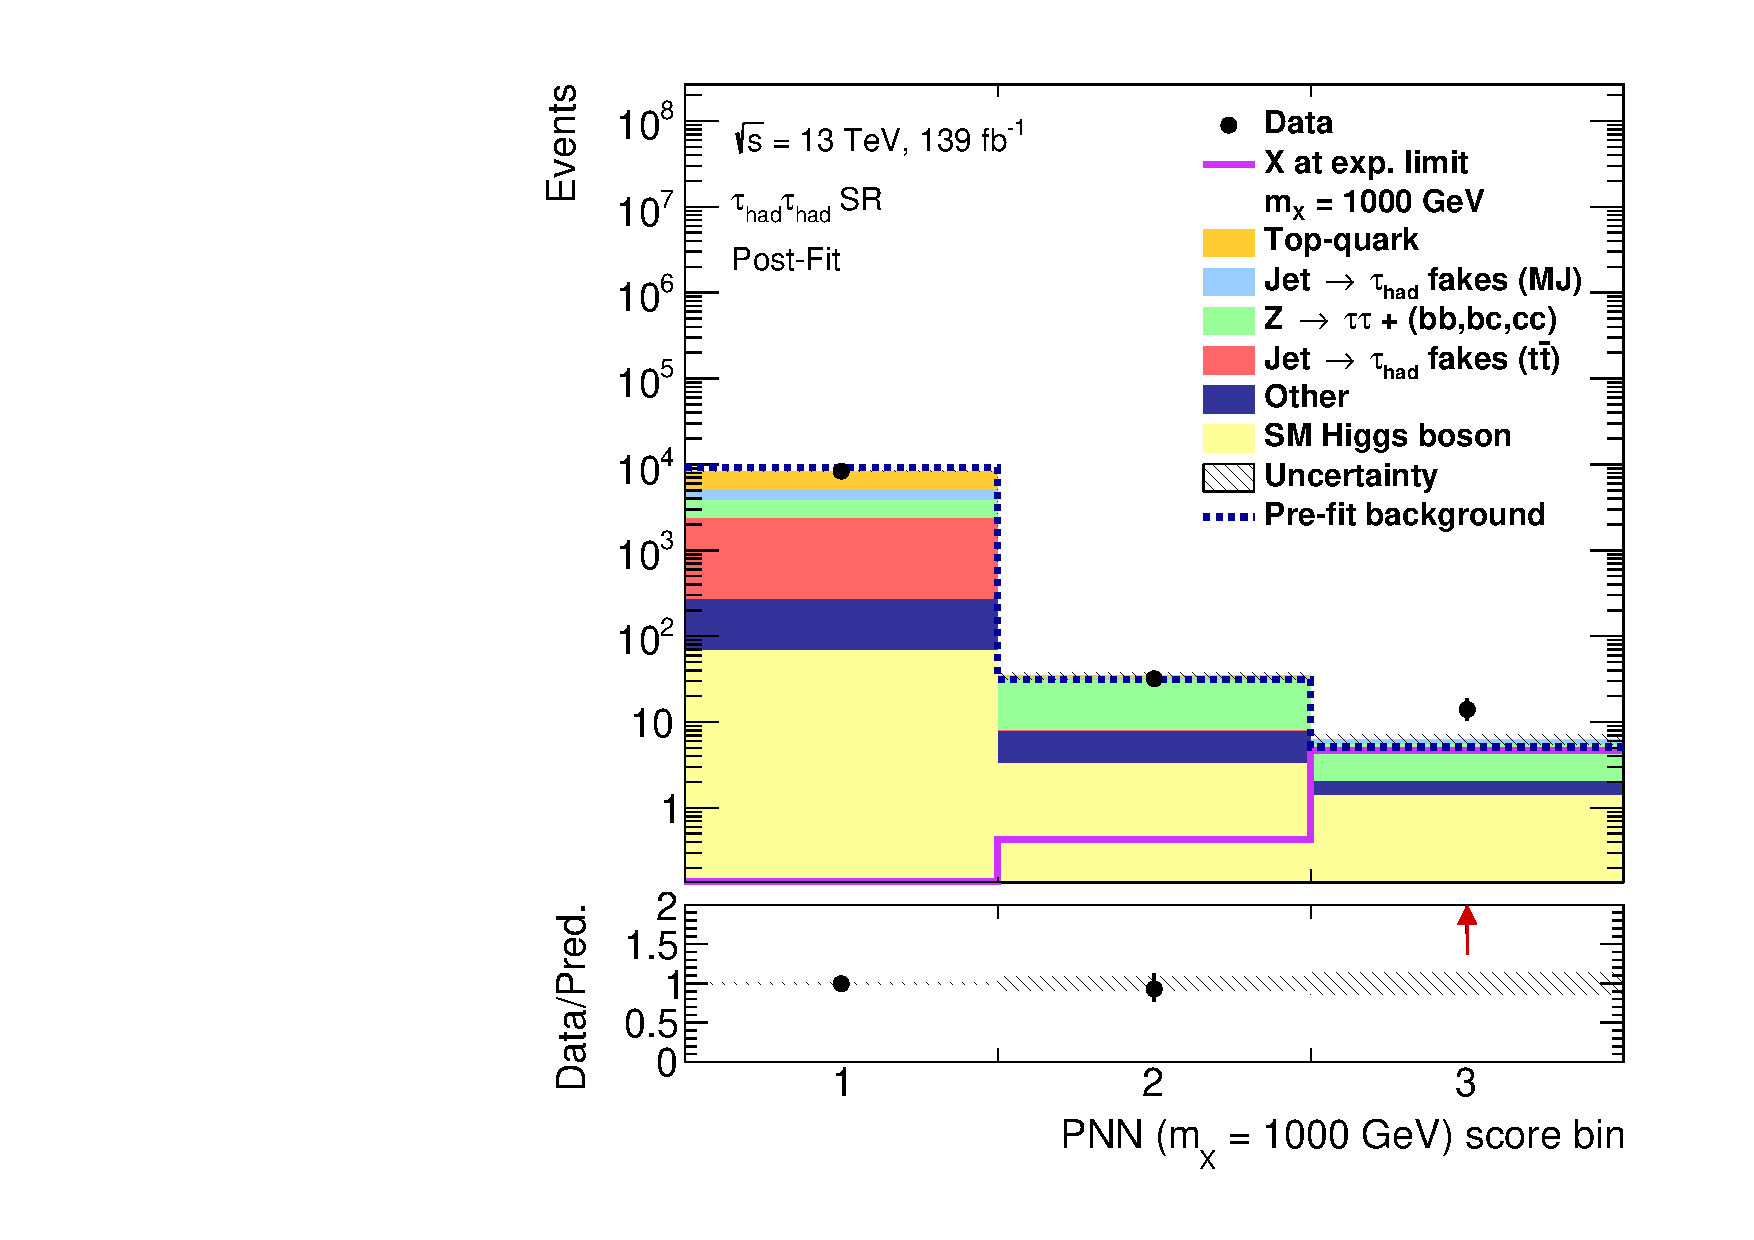
\includegraphics[width=\textwidth]{results_res/postfit/Region_BMin0_incJet1_distPNN1000_J2_Y2015_DLLOS_T2_SpcTauHH_L0_GlobalFit_conditionnal_mu0log}
    \subcaption{$\mX = \SI{1000}{\GeV}$}%
    \label{fig:pnn1000_postfit}
  \end{subfigure}\hfill%
  \begin{subfigure}{0.495\textwidth}
    \centering

    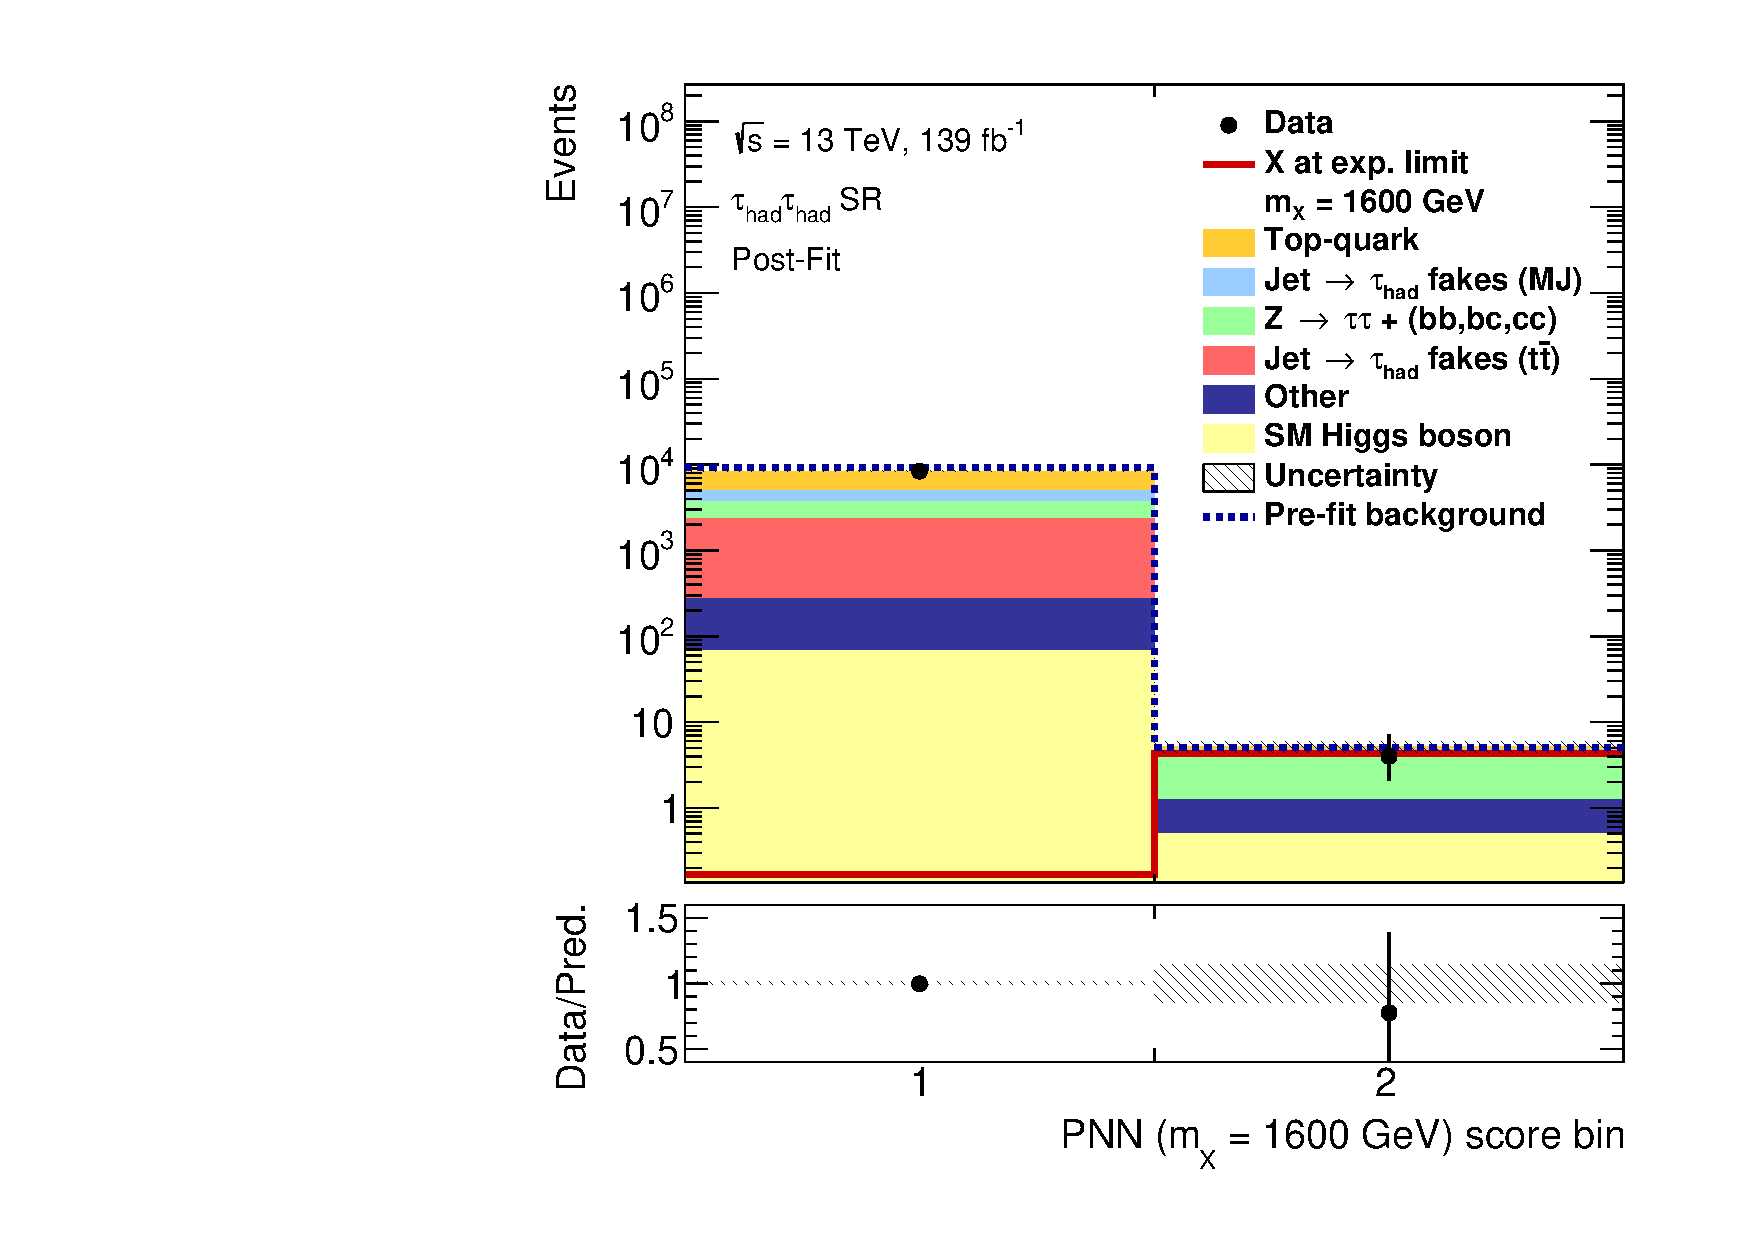
\includegraphics[width=\textwidth]{results_res/postfit/Region_BMin0_incJet1_distPNN1600_J2_Y2015_DLLOS_T2_SpcTauHH_L0_GlobalFit_conditionnal_mu0log}
    \subcaption{$\mX = \SI{1600}{\GeV}$}
  \end{subfigure}

  \caption[Distributions of selected PNN discriminants in the \hadhad channel
  after the background-only fit.]{Distributions of selected PNN discriminants in
    the \hadhad channel after the fit of the background-only model to observed
    data in all regions. The distributions are shown for four different mass
    parameter values of the PNN ranging from \SI{300}{\GeV} to
    \SI{1600}{\GeV}. The signal overlay is scaled to the expected upper limit
    on~$\sigma(pp \to X \to HH)$ for a given \mX.}%
  \label{fig:resonant_mva_postfit}
\end{figure}


\begin{table}[htbp]
  \centering

  \caption[Expected and observed number of events in the \hadhad~SR for
  signal-like bins of the PNN discriminant after the background-only
  fit.]{Expected and observed number of events in the \hadhad~SR for signal-like
    bins of the PNN discriminant after a fit of the background-only fit model to
    observed data in all regions. The two most signal-like bins are shown for
    $\mX = \SI{300}{\GeV}$ and \SI{500}{\GeV}. $\dagger$:~Only the most
    signal-like bin is shown for $\mX = \SI{1000}{\GeV}$ and \SI{1600}{\GeV}.}%
  \label{tab:yields_postfit_resonant}

  \resizebox{\textwidth}{!}{%

    \begin{tabular}{lc
  %@{\hskip 12pt}
  S[table-format=3.2(2)]
  @{\hskip 12pt}
  S[table-format=3.2(2)]
  @{\hskip 12pt}
  S[table-format=3.2(2)]
  @{\hskip 12pt}
  S[table-format=3.2(2)]
  }
  \toprule
  && \multicolumn{4}{c}{Event yield in the most signal-like bin(s)} \\
  \cmidrule{2-6}
  Process                              & $\mX$ & {\SI{300}{\GeV}} & {\SI{500}{\GeV}} & {\SI{1000}{\GeV} ($\dagger$)} & {\SI{1600}{\GeV}  ($\dagger$)} \\
  \midrule
  $X \to HH$ ($\sigma = \SI{1}{\pico\barn}$)
                                       && 18.2 +- 2.9    & 156 +- 16    & 379 +- 38      & 139 +- 28      \\
  \midrule
  Top quark                            && 15.6 +- 2.0    & 2.70 +- 0.44 & 0.12 +- 0.03   & 0.37 +- 0.05   \\
  $Z \to \tautau + (bb,bc,cc)$         && 1.38 +- 0.26   & 7.7 +- 1.1   & 3.50 +- 0.65   & 3.12 +- 0.54   \\
  Single Higgs boson                   && 0.40 +- 0.07   & 2.91 +- 0.61 & 1.40 +- 0.42   & 0.5 +- 0.27    \\
  Jet $\to \faketauhadvis$ (multi-jet) && 5.89 +- 0.92   & 3.48 +- 0.64 & 0.63 +- 0.12   & 0.42 +- 0.07   \\
  Jet $\to \faketauhadvis$ (\ttbar)    && 17.4 +- 2.3    & 1.89 +- 0.28 & 0              & 0              \\
  Other backgrounds                    && 0.21 +- 0.03   & 1.75 +- 0.34 & 0.65 +- 0.13   & 0.74 +- 0.15   \\
  \midrule
  Total background                     && 40.9 +- 3.1    & 20.4 +- 1.9  & 6.29 +- 0.88   & 5.15 +- 0.74   \\
  \midrule
  Observed data                        && 40             & 17           & 14             & 4              \\
  \bottomrule
\end{tabular}

%%% Local Variables:
%%% mode: latex
%%% TeX-master: "../phd_thesis"
%%% End:

  }
\end{table}

The comparison of the PNN distributions after the background-only fit with the
observed data show decent agreement with exception of the PNN discriminant for
resonances with $\mX = \SI{1000}{\GeV}$ shown in~\Cref{fig:pnn1000_postfit}. In
the most signal-like bin of the corresponding PNN distribution 14 events are
observed, while the background-only model predicts a total of \num{6.29 +- 0.88}
events. This represents a large excess in the number of observed events over the
expectation.

% Pvalues
% Comb: 0.0012948798248544335
% Hadhad: 0.00233581755310297
% Lephad: 0.1208430826663971
%
% Significances
% Comb: 3.0126516970870054
% Hadhad: 2.828844777446568
% Lephad: 1.1707826205098675
The background-only and the signal-plus-background models are compared using
tests for the discovery of a signal. The combination of all channels yields an
excess at $\mX = \SI{1000}{\GeV}$ with an observed $p$-value of $\num{1.3e-3}$,
which corresponds to a discovery significance of $\num{3.0}\sigma$.
% \footnote{By convention in HEP the discovery significance is expressed in
% terms of $\sigma$ given by $\Phi^{-1}(1 - p)$, where $\Phi^{-1}$ is the
% inverse cumulative distribution function (quantile function) of the Standard
% Normal distribution and $p$ the $p$-value of the test.}
The excess is localised in the \hadhad~channel with a significance of
$\num{2.8}\sigma$ when restricting the test to the \hadhad~SR and the
\ZHF~CR. The $p$-values and significances for tests of all considered signal
hypotheses are shown in \Cref{fig:local_pvalues}, separately for the \lephad and
\hadhad channels and their combination. The significances quoted thus far do not
account for multiple hypothesis testing and are therefore referred to as
\emph{local significances}. The effect of multiple testing is discussed in
\Cref{sec:global_significance}.

\begin{figure}[htbp]
  \centering

  % Workspaces: comb_2022_01_29
  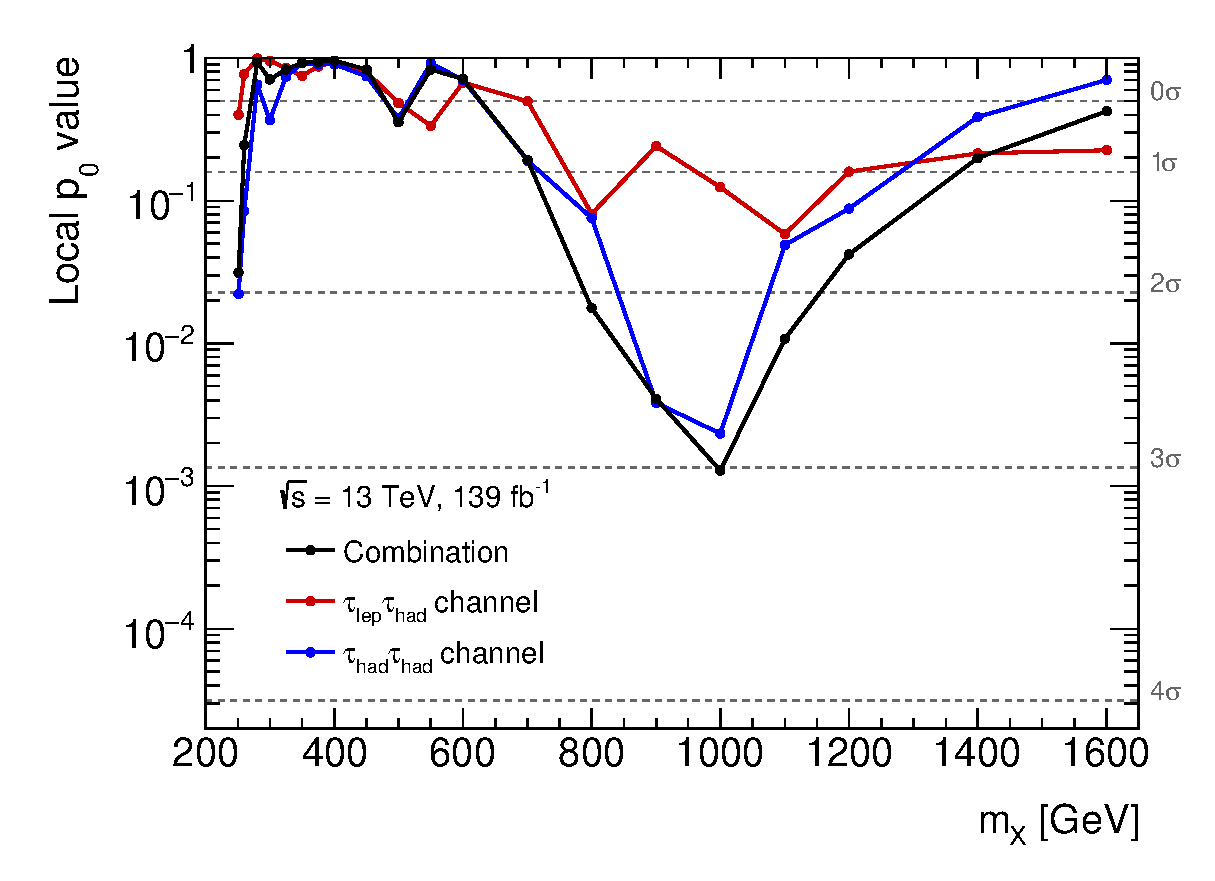
\includegraphics[width=0.6\textwidth]{results_res/resonant_comb_pvalues}

  \caption[Observed local $p$-values of discovery tests performed in the search
  for resonant \HH production.]{Observed local $p$-values for the comparison of
    the background-only and the signal-plus-background model as a function of
    the mass of the resonance. The asymptotic approximation is used for the
    $p$-value computation.}%
  \label{fig:local_pvalues}

  % Dashed lines indiciate the equivalent right-tailed probabilities in
  % terms of standard deviations of a centered Normal distribution,
  % formally given by the condition $p_0 = \mathbb{P}(Z > n \sigma)$
  % for~$Z \sim \mathcal{N}(0, \sigma^2)$ and $n = 0, 1, \dots, 4$.
  % \todo[inline]{Discuss what's going on at 251? At around 400?}
\end{figure}

% Discuss the width of the excess
A broad excess can be observed in~\Cref{fig:local_pvalues} with tests of
resonances with masses in the range of \SIrange{800}{1200}{\GeV} being
significant at the $2\sigma$-level. At mass scales of \SI{1000}{\GeV} a broad
significance response is expected for a true signal primarily for two reasons:
First, the absolute resolution of the \mHH reconstruction degrades with
increasing \mX. Second, the PNNs are not optimised to distinguish between
different signal hypotheses but rather between signal and background, which
leads to additional broadening. \Cref{fig:local_pvalues_injected} compares the
observed significances with the expectation after injecting signals with cross
sections at their best-fit values. These injection tests show that the width of
the observed significance response is in decent agreement with the expectation
for a signal with a mass of about \SI{1000}{\GeV}.
% This effect is further illustrated in \Cref{fig:local_pvalues_injected} where
% the observed local significances are compared to the expectation after
% injecting signals at their best-fit signal strengths. The width of
% significance response of the observed excess is similar to the expectation
% obtained from these injection tests.

\begin{figure}[htbp]
  \centering

  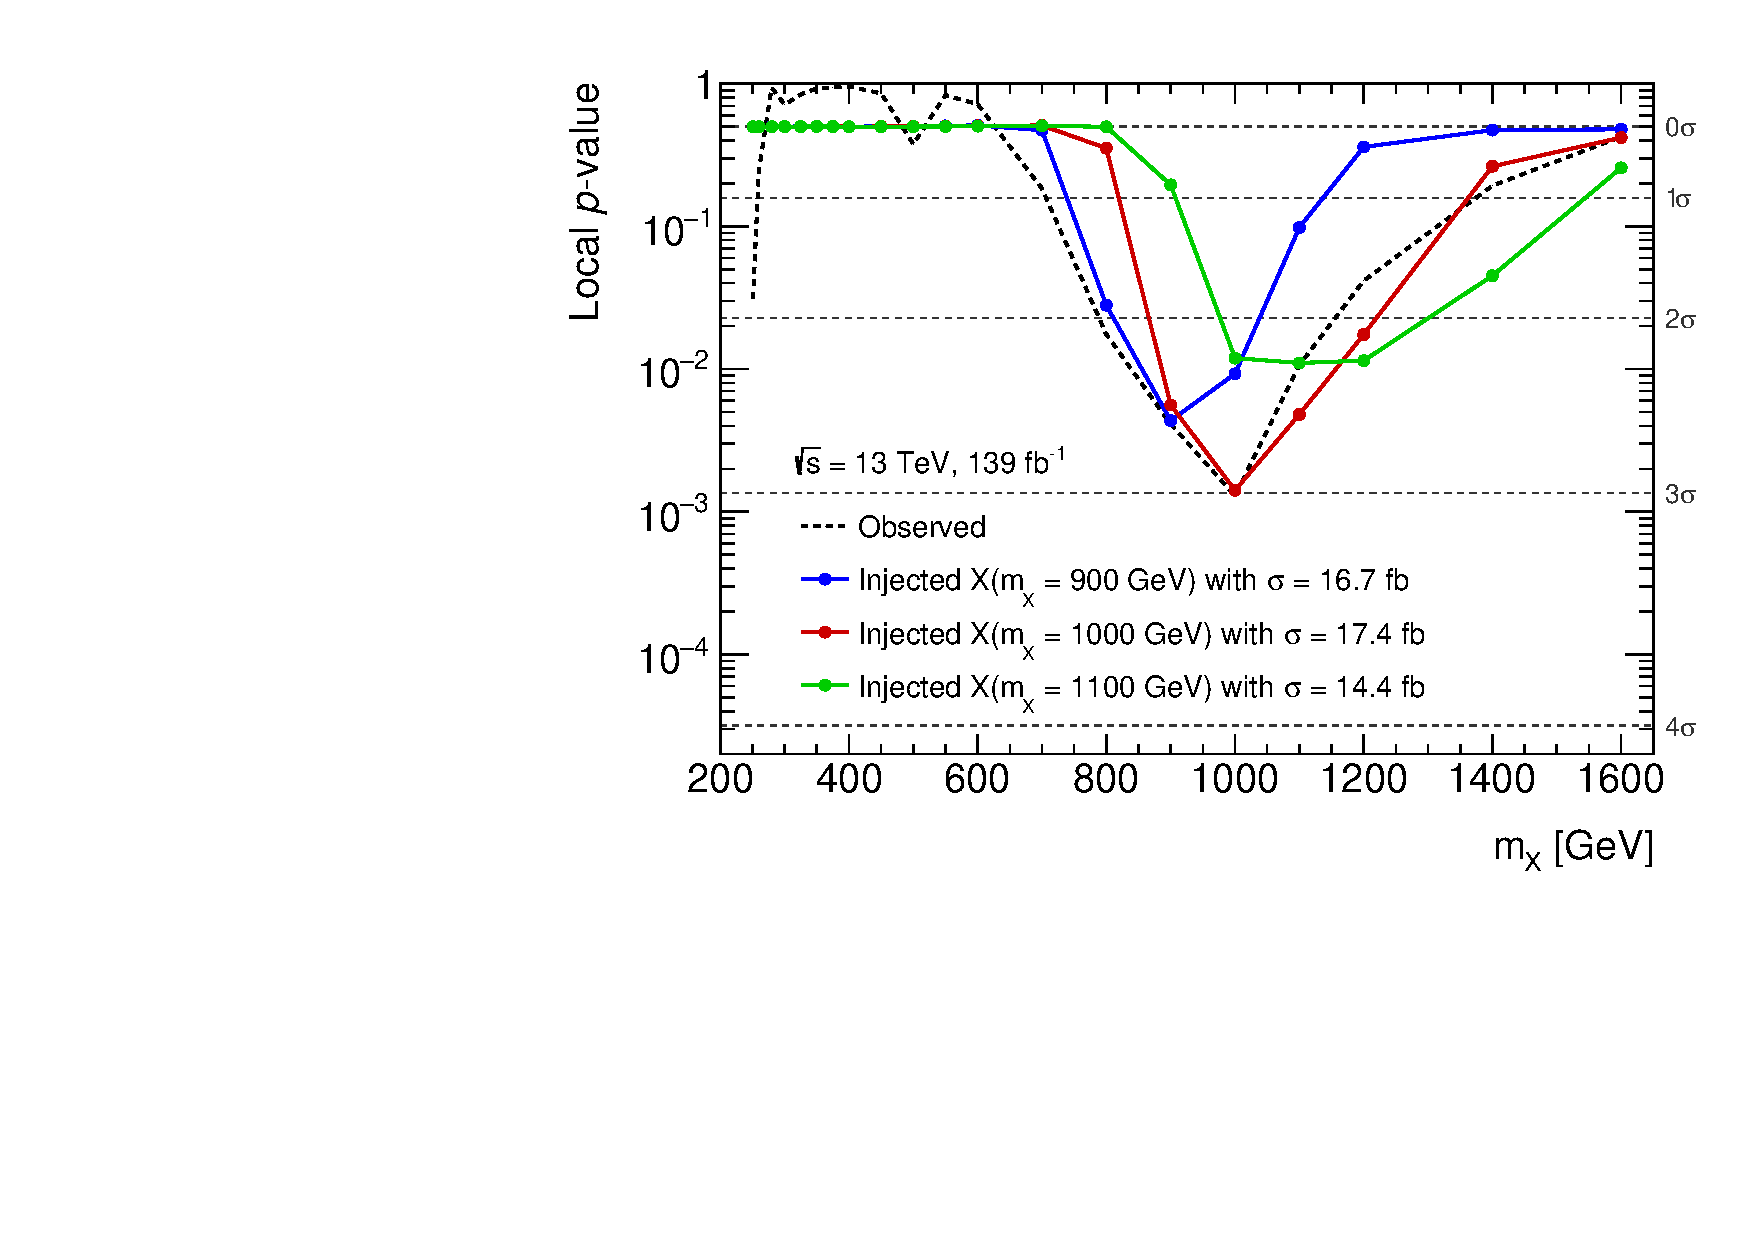
\includegraphics[width=0.6\textwidth]{results_res/injection}

  \caption[Expected local $p$-values of discovery tests performed on Asimov
  dataset with injected signals.]{Expected local $p$-values of discovery tests
    performed on Asimov datasets with injected signals with \mX ranging from
    \SIrange{900}{1100}{\GeV}. The injected signals are normalised to their
    best-fit cross section from the unconditional fit to observed data in all
    regions. The observed $p$-values (dashed line) are shown for comparison.}%
  \label{fig:local_pvalues_injected}
\end{figure}

The best-fit cross section of $pp \to X(\mX = \SI{1000}{\GeV}) \to HH$ obtained
from the fit of the PNN discriminants to observed data in all analysis channels
is~$(\num{17.4}\valuesep^{\hspace{0.25pt}+\hspace{0.25pt}7.5}_{-6.5})\valuesep\si{\femto\barn}$. The
compatibility of the cross section measurement in the \hadhad and \lephad
channels is compared under the assumption of negligible correlation between the
measurements in both channels.
% \footnote{The measurement is limited by the statistical precision of the
% number of observed events which are uncorrelated due to both channels being
% orthogonal.}
While a slight tension at the level of $1\sigma$ is observed, the measurement in
both channels are generally compatible. Further discussion of the excess at
$\mX = \SI{1000}{\GeV}$ is given in
\Cref{sec:global_significance,sec:result_discussion}.

Upper limits are set on $\sigma(pp \to X \to \HH)$ as a function of \mX using
the \CLs method at \SI{95}{\percent} CL. The observed and expected exclusion
limits on the cross section are shown in \Cref{fig:res_upper_limits}. Scalar
resonances produced with a cross sections ranging from
\SIrange{20}{900}{\femto\barn}, depending on \mX, are excluded given the
observed data in all regions. The expected and observed limits are additionally
tabulated in~\Cref{app:limit_tables} for all \mX and separately for the \hadhad
channel, the \lephad channel, and their combination.

\begin{figure}[htbp]
  \centering

  % Workspaces: comb_2022_01_29
  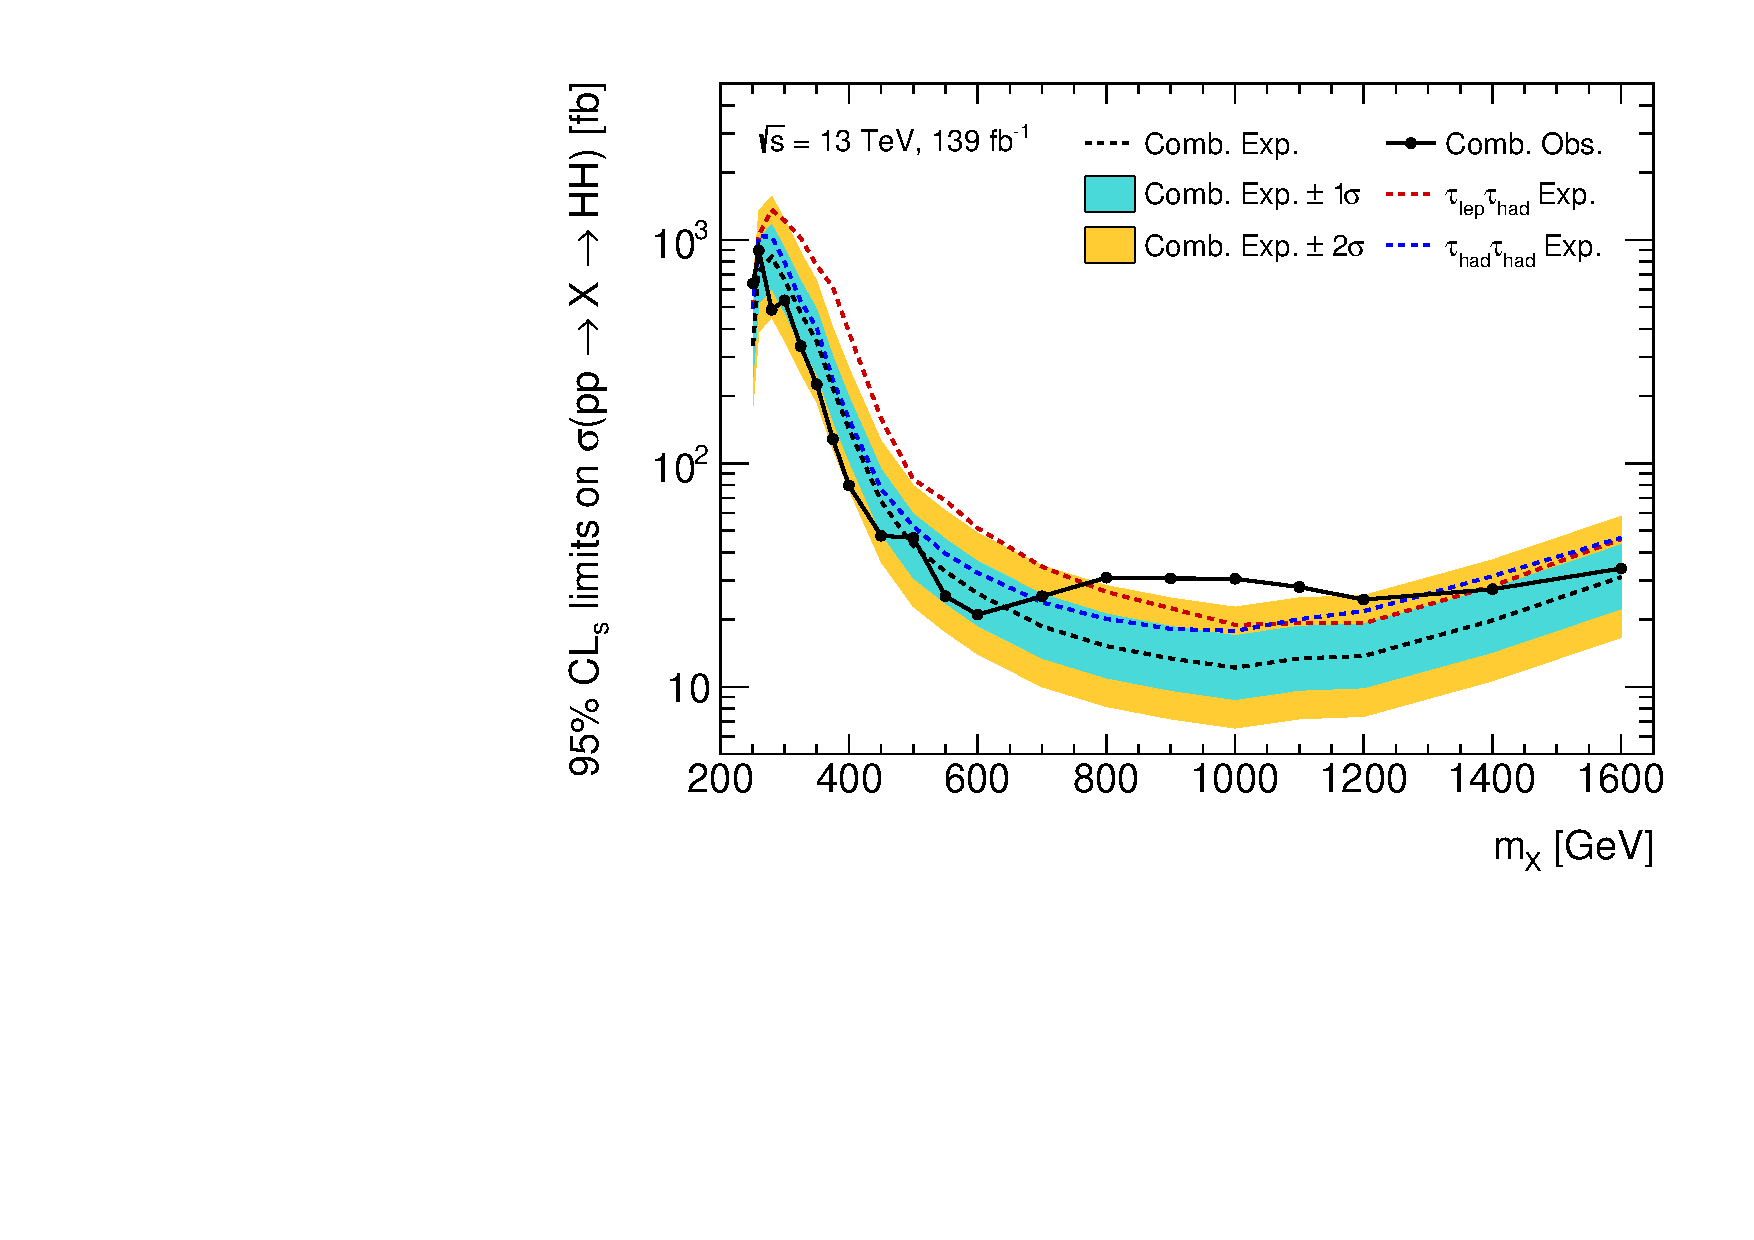
\includegraphics[width=0.6\textwidth]{results_res/resonant_upper_limits}

  \caption[Upper limits on $\sigma(pp \to X \to \HH)$ as a function of the mass
  of the scalar resonance.]{Upper limits on $\sigma(pp \to X \to \HH)$ as a
    function of the mass of the scalar resonance. The exclusion limits are
    obtained using the \CLs method at \SI{95}{\percent} CL. The expected upper
    limits from the \hadhad and \lephad channels are overlayed for comparison.}%
  \label{fig:res_upper_limits}
\end{figure}

The upper limits on the cross section improve quickly in the \mX range from
\SIrange{300}{500}{\GeV} as a consequence of the increasing signal acceptance
and increasing signal-background separation of the PNNs with \mX. In particular,
the ability to distinguish between signal and top-quark backgrounds, which have
a large contribution for $\mX \lesssim \SI{500}{\GeV}$, improves quickly as
larger resonance masses are considered. For $\mX \geq \SI{1000}{\GeV}$, the
upper limits start to degrade due to the inability to resolve the constituents
of the $H \to \tautau$ and $H \to \bbbar$ candidates.

% This is a consequence of the large positive slope in signal acceptance with
% respect to the mass of the scalar resonance
% (cf.~\Cref{fig:signal_acceptance_resonant}) and the increasingly distinct
% signature of the signal aiding in the discrimination between the signal and
% background processes.

% This leads to a broad plateau of the upper limit and a degradation of the
% exclusion limits at the upper end of the considered mass range.

The importance of individual analysis channels to the expected upper limits
varies with the considered resonance mass. Except for the smallest \mX, where
the \hadhad channel has only limited signal acceptance, the \hadhad channel
gives the most stringent limits in the range of low to intermediate \mX. This is
due to the \lephad channels being dominated by the large, irreducible top-quark
background in this regime. For signals with $\mX \gtrsim \SI{1000}{\GeV}$ both
channels are dominated by \Zjets backgrounds in the high PNN score regions and
yield similar exclusion limits.

The search for resonant \HH production is primarily limited by the data
statistical uncertainty, particularly for signals with intermediate to high
\mX. This is illustrated in~\Cref{tab:breakdown_res}, where the variance on the
best-fit cross section from the unconditional fit
%,
% \footnote{The excess for $\mX = \SI{1000}{\GeV}$ induces shifts in the
% (observed) variance breakdown depicted in~\Cref{tab:breakdown_res}, slightly
% inflating data statistical uncertainties while suppressing the impact of most
% systematic uncertainties (the exception being signal modelling uncertainties)
% compared to the
% expectation. In~\Cref{app:breakdown_table}~\Cref{tab:breakdown_res_exp_mu0}
% the decomposition is performed for the expectation of
% $\sigma(pp \to X \to HH) = 0$ for comparison.}
% $\hat{\sigma}$,
is decomposed into categories for four exemplary signal hypotheses. Systematic
uncertainties have a sizeable effect
% on the total variance of $\hat{\sigma}$
only for searches for scalar resonances with low mass. Instrumental
uncertainties, most significantly uncertainties affecting jets, \pTmissAbs, and
\tauhadvis, have the largest impact on the search when the reconstructed Higgs
boson candidates have low transverse momenta, as is the case for signals with
low \mX. Similarly, \faketauhadvis backgrounds and uncertainties related to
their data-driven estimation
% , which are partially included in the background statistical
%uncertainties due to the finite number events in the CRs (and non-multi-jet
%subtraction in the case of the \hadhad channel),
play a more important role at low \mX.

\begin{table}[htbp]
  \centering

  \caption[Breakdown of the variance of $\hat{\sigma}$ by uncertainty category
  for the search for resonant \HH production.]{Breakdown of the variance of
    $\hat{\sigma}$, the MLE of the cross section $\sigma(pp \to X\to HH)$, by
    uncertainty category for the fit to observed data in all regions. The
    decomposition is determined analogously to~\Cref{tab:breakdown_nonres}.}%
  \label{tab:breakdown_res}

  % A similar breakdown based on fits to Asimov data is given in
  % \Cref{tab:breakdown_res_exp_mu0} in \Cref{app:breakdown_table}.

  % Observed breakdown
  \begin{tabular}{
  l
  S[table-format=2.0, table-space-text-pre=\textless, table-column-width=1.6cm]
  S[table-format=2.0, table-space-text-pre=\textless, table-column-width=1.6cm]
  S[table-format=2.0, table-space-text-pre=\textless, table-column-width=1.6cm]
  S[table-format=2.0, table-space-text-pre=\textless, table-column-width=1.6cm]
  }
  \toprule
         & \multicolumn{4}{c}{Explained fraction of variance on $\hat{\sigma}$}\\
         %& \multicolumn{4}{c}{of variance on $\hat{\mu}$}\\
  \cmidrule{2-5}
  Source & {$\SI{300}{\GeV}$} & {$\SI{500}{\GeV}$} & {$\SI{1000}{\GeV}$} & {$\SI{1600}{\GeV}$} \\
  \midrule
  \textbf{Data statistical uncertainty}
         & 58\,\si{\percent} & 81\,\si{\percent} & 86\,\si{\percent} & 82\,\si{\percent} \\
  \textbf{Systematic uncertainties}
         & 42\,\si{\percent} & 19\,\si{\percent} & 14\,\si{\percent} & 18\,\si{\percent} \\
  \hspace{0.8em} Instrumental uncertainties
         & 10\,\si{\percent} & 1\,\si{\percent} & 2\,\si{\percent} & {\textless} 1\,\si{\percent}\\
  \hspace{0.8em} Signal modelling uncertainties
         & 2\,\si{\percent}  & 1\,\si{\percent} & 2\,\si{\percent} & 3\,\si{\percent} \\
  \hspace{0.8em} Background statistical uncertainties
         & 19\,\si{\percent} & 11\,\si{\percent} & 3\,\si{\percent} & 11\,\si{\percent} \\
  \hspace{0.8em} Background modelling uncertainties
         & 14\,\si{\percent} & 6\,\si{\percent} & 7\,\si{\percent} & 4\,\si{\percent} \\
  \midrule
  \hspace{1.6em} -- \hspace{0.2em} Top-quark (incl.\ free normalisation)
         & 3\,\si{\percent} & 2\,\si{\percent} & 1\,\si{\percent} & {\textless} 1\,\si{\percent} \\
  \hspace{1.6em} -- \hspace{0.2em} \ZHF (incl.\ free normalisation)
         & 4\,\si{\percent} & 1\,\si{\percent} & 2\,\si{\percent} & 1\,\si{\percent} \\
  \hspace{1.6em} -- \hspace{0.2em} SM Higgs boson
         & {\textless} 1\,\si{\percent} & 2\,\si{\percent} & 2\,\si{\percent} & 2\,\si{\percent} \\
  \hspace{1.6em} -- \hspace{0.2em} Fake-\tauhadvis
         & 4\,\si{\percent} & {\textless} 1\,\si{\percent} & 1\,\si{\percent} & {\textless} 1\,\si{\percent} \\
  \hspace{1.6em} -- \hspace{0.2em} Other
         & {\textless} 1\,\si{\percent} & {\textless} 1\,\si{\percent} & {\textless} 1\,\si{\percent} & {\textless} 1\,\si{\percent} \\
  \bottomrule
\end{tabular}

%%% Local Variables:
%%% mode: latex
%%% TeX-master: "../phd_thesis"
%%% End:


  % Expected breakdown for Asimov with mu = 0
  % \begin{tabular}{
  l
  S[table-format=2.0, table-space-text-pre=\textless, table-column-width=1.6cm]
  S[table-format=2.0, table-space-text-pre=\textless, table-column-width=1.6cm]
  S[table-format=2.0, table-space-text-pre=\textless, table-column-width=1.6cm]
  S[table-format=2.0, table-space-text-pre=\textless, table-column-width=1.6cm]
  }
  \toprule
         & \multicolumn{4}{c}{Explained fraction of variance on $\hat{\sigma}$}\\
         %& \multicolumn{4}{c}{of variance on $\hat{\mu}$}\\
  \cmidrule{2-5}
  Source & {$\SI{300}{\GeV}$} & {$\SI{500}{\GeV}$} & {$\SI{1000}{\GeV}$} & {$\SI{1600}{\GeV}$} \\
  \midrule
  \textbf{Data statistical uncertainty}
         & 59\,\si{\percent} & 81\,\si{\percent} & 82\,\si{\percent} & 82\,\si{\percent} \\
  \textbf{Systematic uncertainties}
         & 41\,\si{\percent} & 19\,\si{\percent} & 18\,\si{\percent} & 17\,\si{\percent} \\
  \hspace{0.8em} Instrumental uncertainties
         & 10\,\si{\percent} & 1\,\si{\percent} & 1\,\si{\percent} & {\textless} 1\,\si{\percent}\\
  \hspace{0.8em} Signal modelling uncertainties
         & 1\,\si{\percent}  & 1\,\si{\percent} & {\textless} 1\,\si{\percent} & 3\,\si{\percent} \\
  \hspace{0.8em} Background statistical uncertainties
         & 18\,\si{\percent} & 11\,\si{\percent} & 7\,\si{\percent} & 9\,\si{\percent} \\
  \hspace{0.8em} Background modelling uncertainties
         & 12\,\si{\percent} & 7\,\si{\percent} & 10\,\si{\percent} & 5\,\si{\percent} \\
  \midrule
  \hspace{1.6em} -- \hspace{0.2em} Top-quark (incl.\ free normalisation)
         & 3\,\si{\percent} & 2\,\si{\percent} & 1\,\si{\percent} & {\textless} 1\,\si{\percent} \\
  \hspace{1.6em} -- \hspace{0.2em} \ZHF (incl.\ free normalisation)
         & 3\,\si{\percent} & 1\,\si{\percent} & 3\,\si{\percent} & 2\,\si{\percent} \\
  \hspace{1.6em} -- \hspace{0.2em} SM Higgs boson
         & {\textless} 1\,\si{\percent} & 2\,\si{\percent} & 3\,\si{\percent} & 2\,\si{\percent} \\
  \hspace{1.6em} -- \hspace{0.2em} Fake-\tauhadvis
         & 4\,\si{\percent} & {\textless} 1\,\si{\percent} & 1\,\si{\percent} & 1\,\si{\percent} \\
  \hspace{1.6em} -- \hspace{0.2em} Other
         & {\textless} 1\,\si{\percent} & {\textless} 1\,\si{\percent} & {\textless} 1\,\si{\percent} & {\textless} 1\,\si{\percent} \\
  \bottomrule
\end{tabular}

%%% Local Variables:
%%% mode: latex
%%% TeX-master: "../phd_thesis"
%%% End:

\end{table}

% \todo[inline]{Ranking plots: Selected masses combined only?}

% \todo[inline]{Table of lephad yields?}

\subsection{Global Significance Estimation in the Search for Resonant \HH
  Production}%
\label{sec:global_significance}

In the search for resonant \HH production, multiple hypothesis tests are
performed, probing a total of 20 different signal hypotheses. When performing
multiple tests, it needs to be considered that under the background-only
hypothesis any test could yield a statistically significant result by chance,
which would constitute a false discovery (type I error). As the number of tests
increases, so does the probability of making one or more false discoveries when
not controlling for this effect. The previously quoted significance of
$3.0\sigma$ of the test at $\mX = \SI{1000}{\GeV}$ does not account for multiple
testing; therefore, the significance was referred to as the local
significance. In this section, an alternative test statistic referred to as the
\emph{global significance} is introduced that controls for the false discovery
rate over a set of hypothesis tests.

The probability of making one or more false discoveries over a set (family) of
hypothesis tests is referred to as the family-wise error rate
(FWER)~\cite{lehmann2005testing}. The FWER can be controlled by setting the
critical thresholds of individual hypothesis tests such that the FWER remains at
an acceptable level. In HEP this is conventionally done by defining the global
$p$-value
\begin{align*}
  \pglobal = \mathbb{P}( \Zmaxlocal > \zmaxlocalobs \mid H_0 )\,\text{,}
\end{align*}
where \Zmaxlocal is the random variable denoting the maximum local significance
over all tests, \zmaxlocalobs is the value of \Zmaxlocal observed in data, and
$H_0$ refers to the background-only hypothesis. The global significance is then
defined as
\begin{align*}
  \zglobal = \Phi^{-1}(1 - \pglobal) \,\text{,}
\end{align*}
where $\Phi^{-1}$ is the quantile function of the Standard Normal
distribution. By convention, discovery is claimed if \pglobal (\zglobal) is less
(greater) than \num{2.87e-7} ($5\sigma$), which ensures that the FWER is at most
\num{2.87e-7}.

The distribution of \Zmaxlocal under the background-only hypothesis is required
to estimate the global significance. In general, this distribution is unknown
and needs to be determined by simulation. This is done as follows:~First, a toy
experiment is drawn from the background-only model. Second, the set of
hypothesis tests is performed for a given toy experiment and the maximum local
significance over all tests is determined. These steps are repeated $N$ times
yielding a sample of realisations of \Zmaxlocal under the background-only
hypothesis. For a given value of \zmaxlocalobs, the global $p$-value can then be
estimated according to
% \begin{align*}
%   \pglobal \approx
%   \frac{
%   \text{Number of toys with } \zmaxlocal > z_{\text{local, obs}}^{\text{max}}
%   }{
%   N
%   } \,\text{,}
% \end{align*}
\begin{align*}
  \pglobal \approx \frac{1}{N} \,\times\, \text{Number of toys with } \zmaxlocal > z_{\text{local, obs}}^{\text{max}} \,\text{,}
\end{align*}
where \zmaxlocal refers to the realisation of \Zmaxlocal for a given toy
experiment. Other methods of calculating global significances exist, see for
example Ref.~\cite{Gross:2010qma}; however, they also rely on the ability of
drawing toy experiments from the background-only model.

In the search for resonant \HH production, the primary difficulty in estimating
the global significance lies in the generation of toy experiments from the
background-only model. While the likelihood functions used for the statistical
interpretation are built based on probabilistic models of the binned PNN
discriminants, these models only provide a description of the discriminants for
a single mass point. However, a background model that jointly describes all
discriminants is required to generate toy experiments for the global
significance estimation. The need for such a model was already indicated by the
large width of the significance response in the signal injection tests
(cf.~\Cref{fig:local_pvalues_injected}), which is caused by a partial overlap of
events selected by the most signal-like bins of the PNN discriminants for
adjacent mass points.

A substitute background-only model is constructed that accounts for dependencies
between all observables entering the statistical interpretation. The model is
constructed such that it closely approximates (after marginalising out
observables not relevant for a given mass point) the background-only models used
for the statistical interpretation in \Cref{sec:results_res}. This ensures that
the same statistical analysis can be applied to toy experiments without
introducing biases due to a mismatch between models. A detailed description of
the substitute model developed for this thesis is given in
\Cref{app:toy_generation}; however, the key parts are highlighted here.

The model is constructed from the pre-fit expectation for all backgrounds except
for the \ttbar and \ZHF normalisation factors, which are set to approximate
post-fit values of 0.97 and 1.35, respectively. The model is divided into three
parts, each part describing a certain type of random variable:
\begin{description}

\item[Observables] Observables are random variables representing the number of
  events that are observed in a given bin (i.e.~$n_{cb}$ in
  \Cref{eq:likelihood_histfactory}). The marginal distributions of the
  observables are Poisson distributions with known expected value under the
  background-only hypothesis. When only considering a single PNN discriminant,
  these observables are mutually independent due to all bins being pairwise
  disjoint. However, this is not the case when considering the PNN discriminants
  for all 20 values of \mX. In this case, the joint distribution of all
  observables is a multivariate Poisson distribution with non-trivial
  dependencies between observables.

  The joint distribution of observables is estimated as follows:~First, the
  marginal distributions of the observables are extracted from the nominal
  background-only models. Second, the linear correlation coefficients for all
  pairs of observables are estimated using MC simulation and CR data, yielding
  correlation matrices for the observables. Lastly, the marginal distributions
  of the observables are linked using a Gaussian copula to form the joint
  distribution of all observables,\footnote{This approach is motivated by
    Sklar's theorem~\cite{Sklar1959FonctionsDR}, which states that any
    $n$-dimensional joint distribution function can be factorised into
    $n$~one-dimensional marginal distribution functions and an $n$-dimensional
    copula~\cite{nelsen}. The copula describes the dependencies between the
    random variables.} where the Gaussian copula is defined by the correlation
  matrix estimated in the second step. Methods of drawing random variates from
  the joint distribution described by the marginals and the Gaussian copula
  exist~\cite{nelsen} and are used for the generation of toy experiments.

\item[Global observables (Barlow--Beeston method)] The global observables
  related to the simplified Barlow--Beeston method are random variables that
  describe the effective number of events from simulation or CR data
  in a given bin (i.e.~$m_{cb}$ in
  \Cref{eq:likelihood_histfactory_constraints}). Similar to the observables, the
  effective number of events has non-trivial dependencies between
  bins of different discriminants. Resampling techniques are applied to MC
  simulations and CR data to produce alternative datasets for background
  estimation. Subsequently, the effective number of events is
  recalculated for every bin using the resampled datasets. The resulting values
  of the global observables are then used as part of the toy experiments.

\item[Global observables (other systematic uncertainties)] The global
  observables related to all other systematic uncertainties (i.e.~$a_p$ in
  \Cref{eq:likelihood_histfactory_constraints}) are assumed to be fully
  correlated for all hypothesis tests and are drawn from the Standard Normal
  distribution.

\end{description}
The statistical model used in the \ZHF~CR is the same for all hypothesis tests;
therefore, standard toy generation methods are used for the observables and the
global observables related to the Barlow--Beeston method in the \ZHF~CR.

% MOVED THESE TO APPENDIX
%
% \subsubsection{Generation of Toy Observables}
%
% \subsubsection{Generation of Toy Global Observables}%
%
% -> appendix/toys.tex


\subsubsection{Sampling Distribution of the Discovery Test Statistic}

Before proceeding with the estimation of the global significance, the validity
of the asymptotic approximation used to determine local significances from
observed values of the $q_0$ test statistic
% , i.e.~$z_{\text{local}} = \sqrt{q_0}$,
is examined. For this purpose, separate sets of toy experiments are generated
using standard toy generation methods.
% Standard methods can be used because the modelling of dependencies between
% tests is not required when determining the sampling distribution of the test
% statistic at the level of an individual hypothesis test.
The quality of the approximation is investigated for all 20 hypothesis tests
using \num{100000} toy experiments per test.
% such that the region close to the threshold of interest of $q_0 \approx 9$
% ($z_{\text{local}} \approx 3$) is well-populated.
A representative example of the $q_0$~sampling distribution under the
background-only hypothesis and the resulting relationship between $q_0$ and the
local significance is shown in~\Cref{fig:q0_samplingdist} and compared to the
asymptotic approximation.

\begin{figure}[htbp]
  \centering

  \begin{subfigure}{0.485\textwidth}
    \centering

    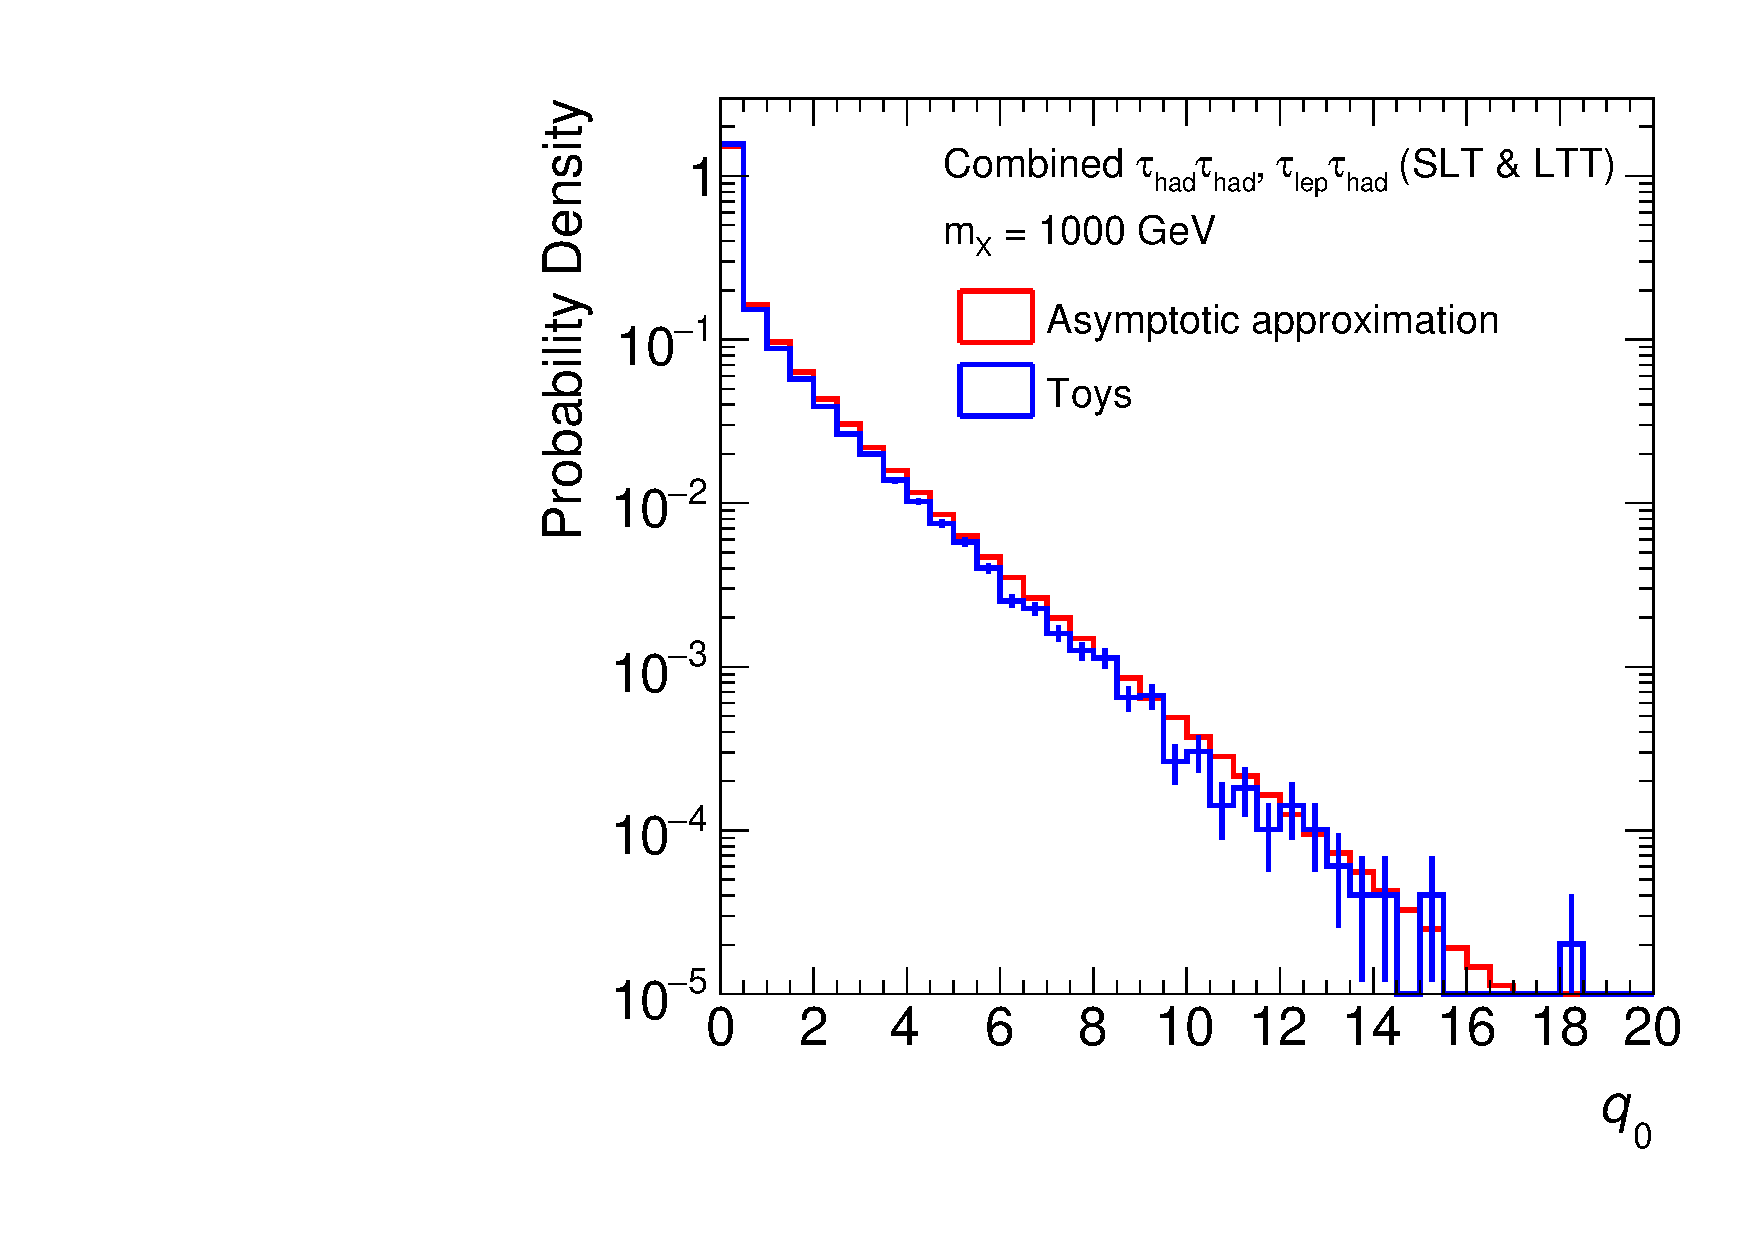
\includegraphics[width=0.95\textwidth, trim=0 0.4cm 0 0, clip]{global_significance/local_sig_toys/q0_1000}
    \subcaption{}
  \end{subfigure}\hfill%
  \begin{subfigure}{0.485\textwidth}
    \centering

    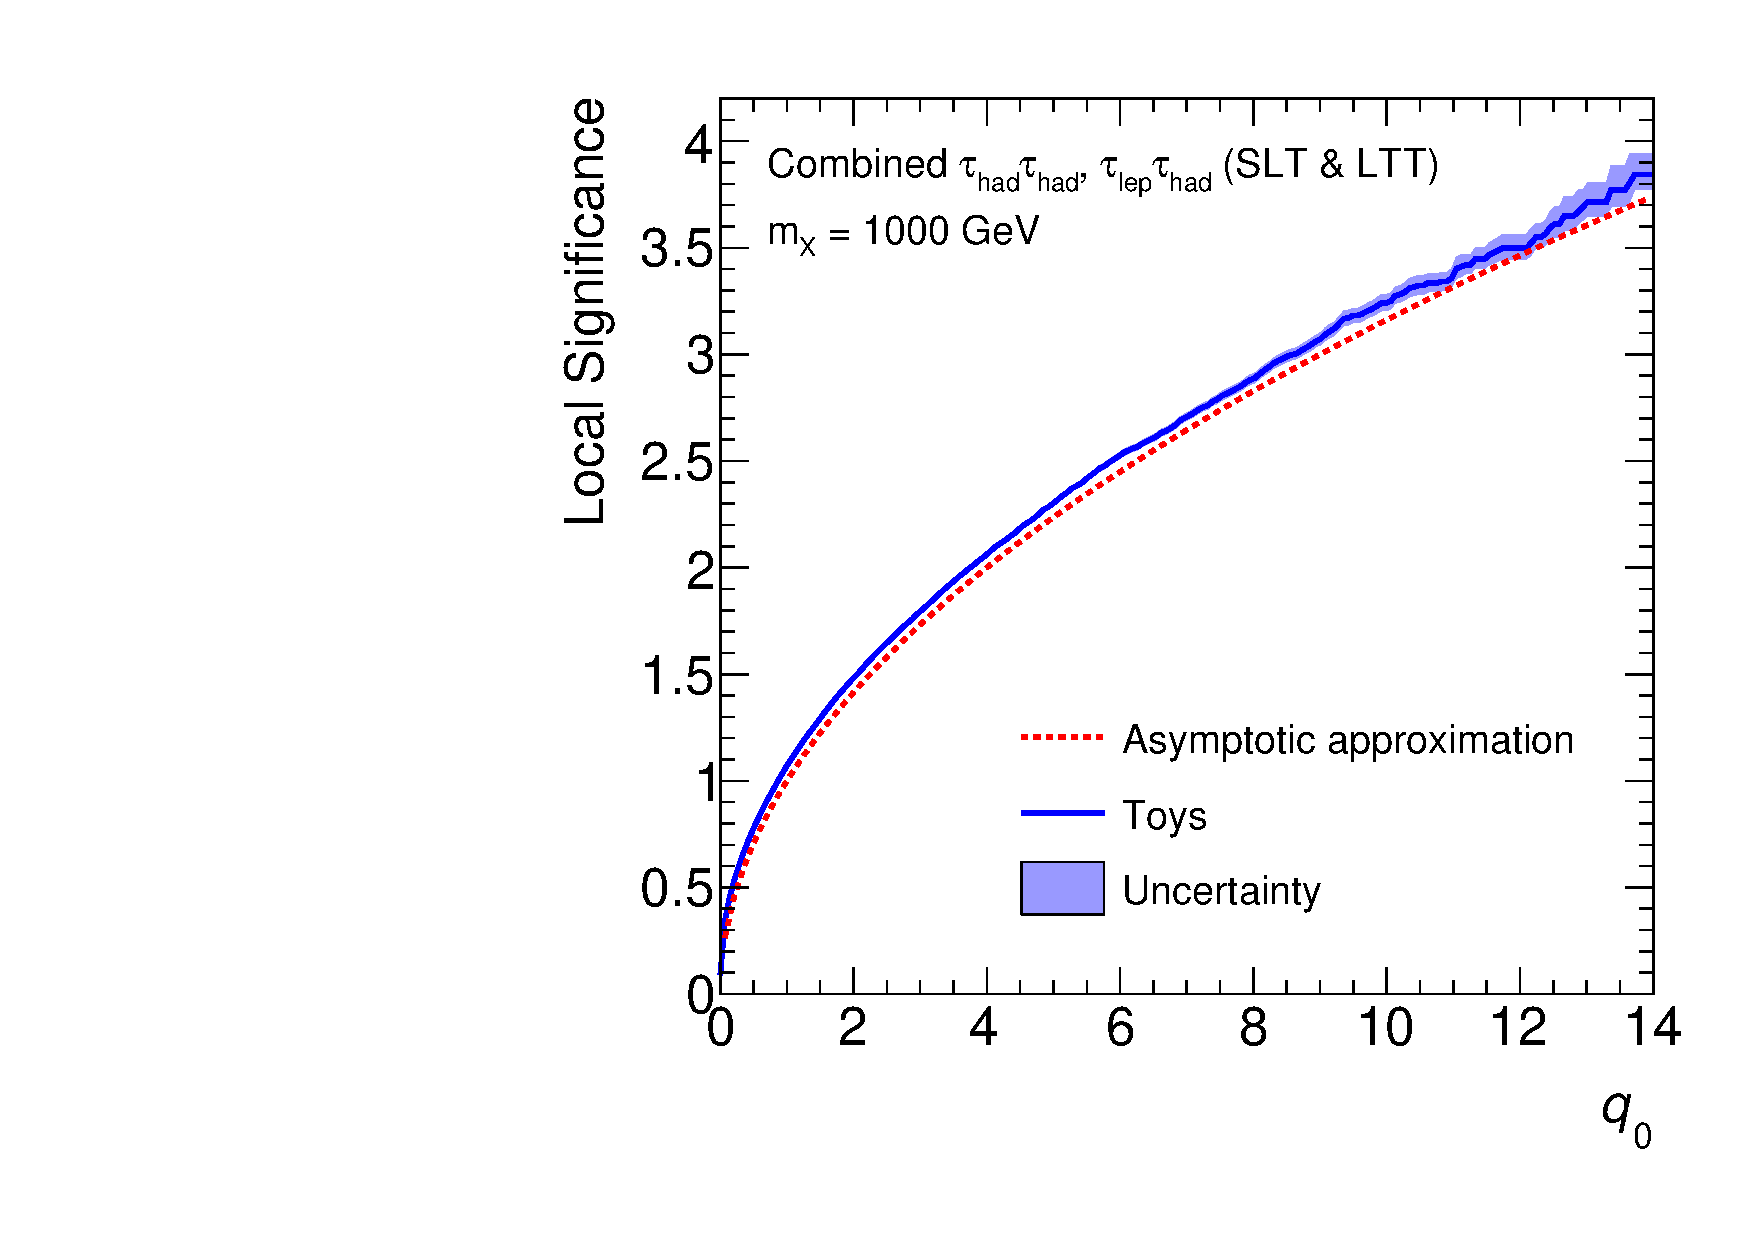
\includegraphics[width=0.95\textwidth, trim=0 0.4cm 0 0, clip]{global_significance/local_sig_toys/q0sig_1000}
    \subcaption{}%
    \label{fig:q0_samplingdist_q0sig}
  \end{subfigure}

  \caption[Comparison of the $q_0$ sampling distribution under the
  background-only hypothesis for the asymptotic approximation and a toy-based
  estimate.]{Comparison of the $q_0$ sampling distribution under the
    background-only hypothesis for the asymptotic approximation and an estimate
    using \num{100000} toy experiments (a). The resulting relationship between
    the local significance and the observed value of $q_0$ (b). Both are shown
    for the test of the $\mX = \SI{1000}{\GeV}$ signal hypothesis combining all
    analysis channels.}%
  \label{fig:q0_samplingdist}
\end{figure}

The asymptotic approximation provides a good description of the relationship
between $q_0$ and $z_{\text{local}}$ for all 20 hypothesis tests considered in
the search for resonant \HH production. Both methods of estimating the local
significance agree within a few percent for all hypothesis tests. Nevertheless,
toy-based estimates are used for the global significance estimation. In this
case, the local significance of the excess at $\mX = \SI{1000}{\GeV}$ with
$q_0 = \num{9.08}$ is estimated to be $\num{3.09 +- 0.03}$, which is obtained
from~\Cref{fig:q0_samplingdist_q0sig}.

% The excess observed in data for the test of the $\mX = \SI{1000}{\GeV}$
% hypothesis yields a value of $q_0 = \num{9.08}$ for the combination of all
% channels. This value of the discovery test statistic corresponds to a local
% significance of $\num{3.01}$ under the asymptotic approximation and
% $\num{3.09 +- 0.03}$ for the toy-based estimate depicted
% in~\Cref{fig:q0_samplingdist_q0sig}. The following analysis of the global
% significance proceeds using toy-based estimates of local significances.
%
% \footnote{For the purpose of determining the global significance,
%   the differences between the asymptotic approximation and the toy-based
%   estimate of the $q_0$ sampling distributions have negligible impact on the
%   result.}

% ----------------------------------------------------------------------------
\subsubsection{Global Significance Estimation}

% In the following the determination of the global significance is discussed
% using toy experiments drawn from the background-only model introduced in the
% previous sections. The likelihood functions used to perform the discovery
% tests are structurally identical to the ones used to obtain the primary
% results (cf.\ \Cref{sec:statistical_analysis}) only replacing the values of
% observables and global observables with the ones drawn from the model.

A total of \num{10000} toy experiments are performed that use observables and
global observables drawn from the substitute background-only model outlined
previously.
% The number of toy experiments is chosen such that the global significance can
% be estimated with a statistical uncertainty below \num{0.1}.  This choice is
% based on the expectation of a global significance close to $2$, which is
% obtained from the assumption that all 20 tests are mutually independent.
The following steps performed for every toy experiment:
\begin{enumerate}

\item The values of $q_0$ are determined for all 20 hypothesis tests considered
  in the analysis. This step involves performing a conditional (background-only)
  and an unconditional maximum likelihood fit of the model parameters after
  replacing observables and global observables in the likelihood functions with
  values from the toy experiment.

\item The observed values of $q_0$ are translated into local significances using
  the toy-based estimates of the relationship between $q_0$ and
  $z_{\text{local}}$.

\item The maximum local significance over all tests is determined.

\end{enumerate}
% Performing these steps for all toy experiments yields an estimate of the
% distribution of \Zmaxlocal under the background-only hypothesis.

The fits required to obtain the discovery test statistic do not always
succeed. A total of \num{74} fits\footnote{Out of \num{400000} fits, i.e.\
  $20\,\text{(number of tests)} \times 2\,\text{(conditional \& unconditional
    fit)} \times \num{10000}\,\text{(number of toys)}$.}  did not converge even
after retrying with altered optimiser settings. The failures are restricted to
unconditional fits in cases where a large deficit is observed in a bin with
large signal sensitivity. In these cases, the value of $q_0$ is set to 0 since a
deficit does not constitute evidence in favour of the signal-plus-background
hypothesis.
% These failures do not occur randomly but systematically, being restricted to
% failures of unconditional fits for cases where a large deficit is observed in
% the toy data of a bin with large signal sensitivity. Since a deficit does not
% constitute a discovery in this search, the value of $q_0$ is set to 0 in these
% cases and the toy experiment is kept.

The result of the toy experiments is shown in~\Cref{fig:zmax_toys}, which
illustrates the effect of multiple hypothesis testing leading to an expectation
of \Zmaxlocal of about \num{1.8} even in the absence of a signal. The toy
experiments yield an estimate of the global $p$-value of
\begin{align*}
  \pglobal = \num{0.0222}\numerrt{0.0015}{toy stat.}
\end{align*}
and an equivalent global significance of
\begin{align*}
  \zglobal = \num{2.01}\numerrt{0.03}{toy stat.} \,\text{,}
\end{align*}
where only statistical uncertainties from the finite number of toy experiments
for the global significance estimation are considered. In addition, the
statistical uncertainty of the toy-based estimate of the relationship between
$q_0$ and $z_{\text{local}}$ is propagated to the global significance using the
bootstrap method~\cite{10.1214/aos/1176344552,efron1994introduction}. The
resulting uncertainty on $z_{\text{global}}$ is \num{0.04} yielding a final
result of
\begin{align*}
  \zglobal = \num{2.01}\numerrt{0.05}{total} \,\text{.}
\end{align*}

\begin{figure}[htbp]
  \centering

  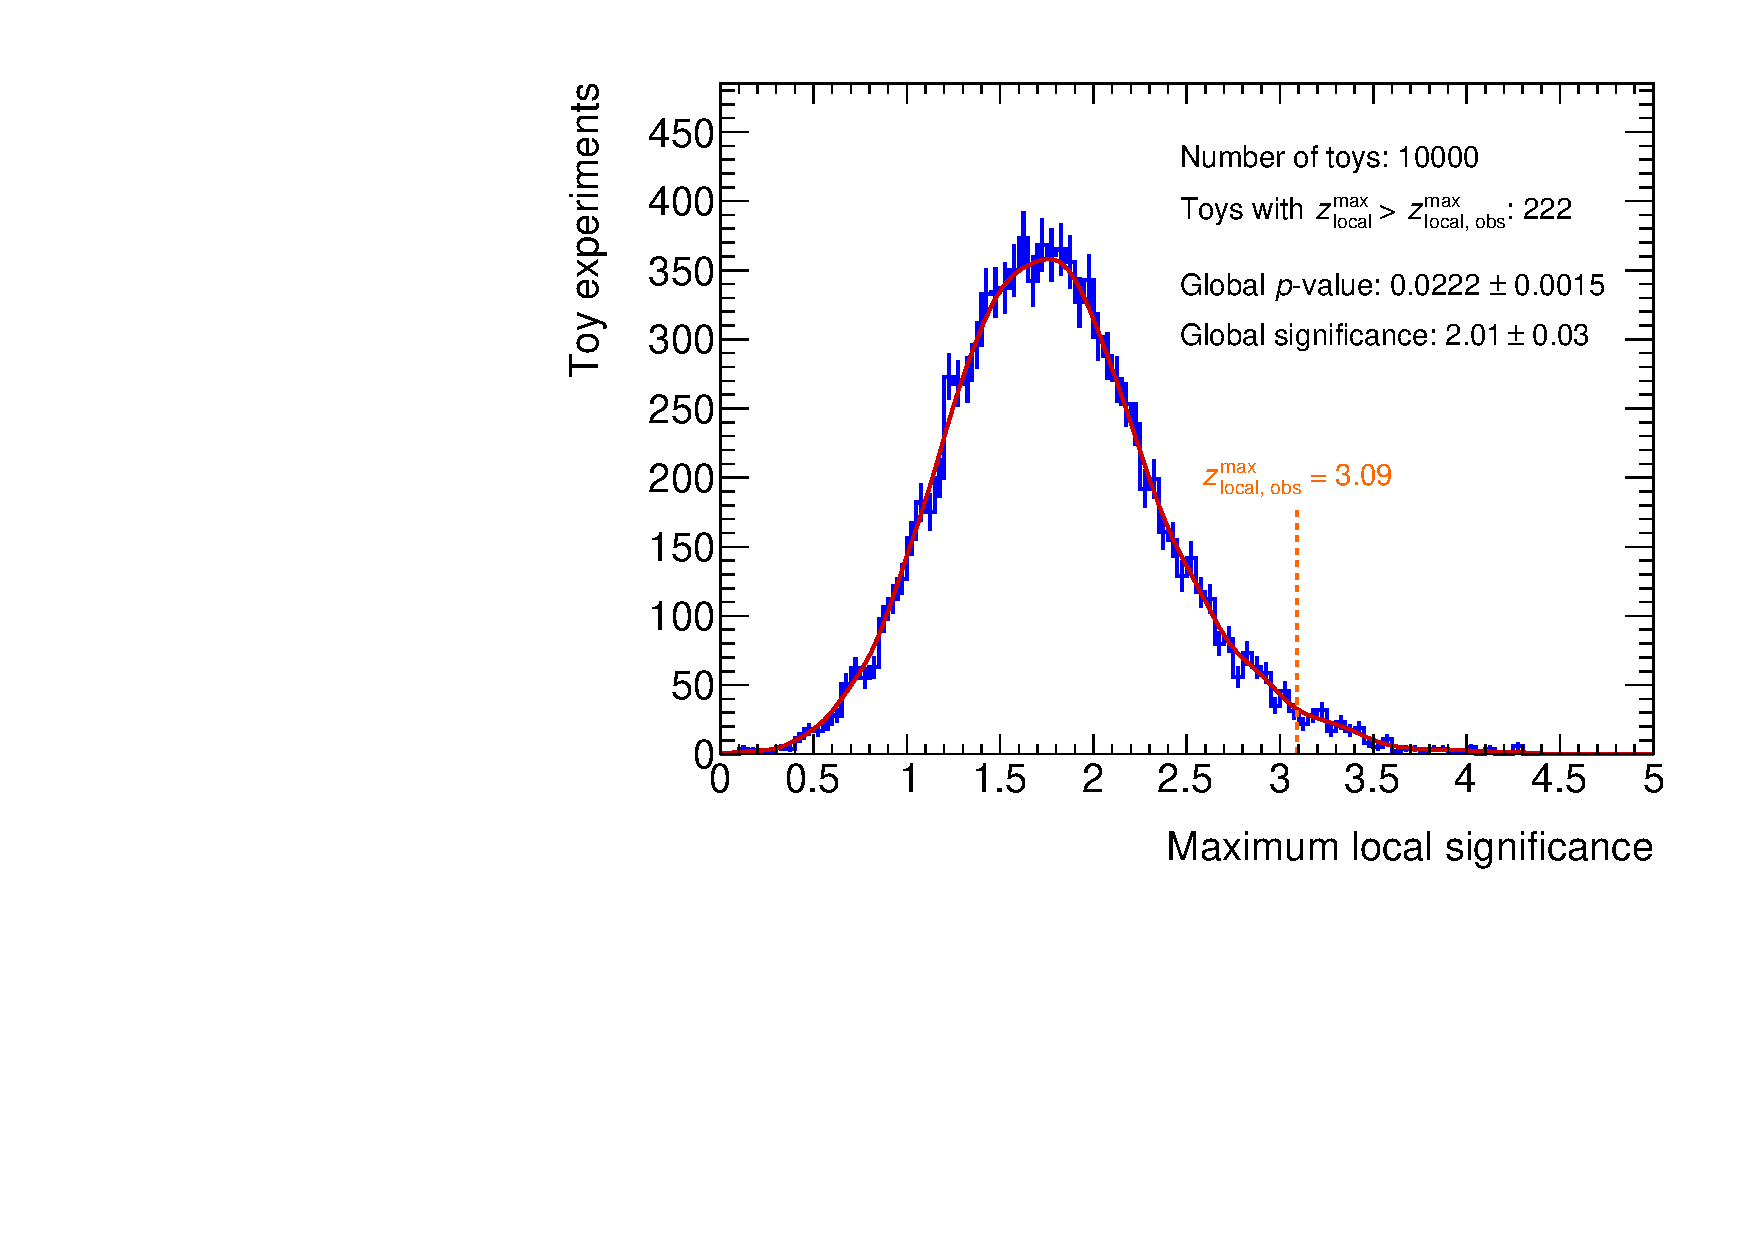
\includegraphics[width=0.6\textwidth]{global_significance/zmax_toys}

  \caption[Toy-based estimate of the distribution of the maximum local
  significance under the background-only hypothesis.]{Toy-based estimate of the
    distribution of the maximum local significance, \Zmaxlocal, under the
    background-only hypothesis. The local significance of the largest excess
    observed in data is indicated in orange. The distribution after kernel
    smoothing is overlayed in red for illustration purposes. The uncertainty on
    the global $p$-value/significance only accounts for the finite number of toy
    experiments.}%
  \label{fig:zmax_toys}
\end{figure}

Lastly, the toy experiments can be used to estimate the correlations between
local significances for all tests under the background-only hypothesis. For this
purpose, a signed definition of the local significance given by
\begin{align*}
  z_{\text{local}}^{\text{signed}} = \sgn(\hat{\sigma}) \sqrt{q_0}
\end{align*}
is used, where $\sgn(\hat{\sigma})$ refers to the sign of the best-fit cross
section. This choice is made for easier interpretation since
$z_{\text{local}}^{\text{signed}}$ follows a Standard Normal distribution under
the background-only assumption. The correlation matrix between
$z_{\text{local}}^{\text{signed}}$ for all 20 hypothesised values of \mX is
shown in \Cref{fig:corr_sig}. The figure illustrates the increasing correlation
between tests at large \mX that was previously observed in the signal injection
tests.

\begin{figure}[htbp]
  \centering

  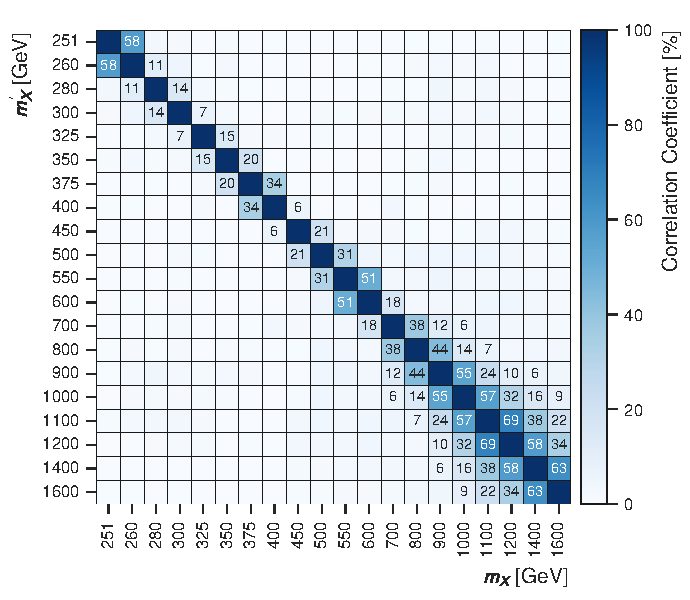
\includegraphics[width=0.65\textwidth]{global_significance/sig_corr}

  \caption[Correlation coefficient between the local significances of discovery
  tests for a signal with mass $\mX$ and $\mX^\prime$ under the background-only
  hypothesis.]{Linear correlation coefficients between the signed local
    significances of hypothesis tests testing the discovery of a signal with
    mass $\mX$ and $\mX^\prime$ under the background-only hypothesis. The
    coefficients are estimated using \num{10000} toy experiments drawn from the
    background-only substitute model. Cells are annotated, omitting the
    diagonal, if the correlation coefficient is greater than or equal to
    \SI{5}{\percent}.}%
  \label{fig:corr_sig}
\end{figure}

% Finally, the result of the toy-based estimation of the global significance
% yielding $z_{\text{global}} = \num{2.01 +- 0.05}$ is compared to case assuming
% that the hypothesis tests can be seen as mutually independent. With this
% simplification the global significance is analytically estimated to be
% \num{2.06 +- 0.04}, using the observed maximum local significance of \num{3.09
% +- 0.03}, which is compatible with the result based on toy experiments. This
% result might seem surprising given the large correlation between tests at high
% \mX shown in~\Cref{fig:corr_sig}, however, this finding is supported by
% simulation. Assuming the joint distribution of signed local significances is
% multivariate Normal with zero mean and covariance matrix given
% by~\Cref{fig:corr_sig}, the global significance can be estimated from
% simulation with negligible statistical precision and compared to the result
% assuming independence. The difference in global significance estimates between
% both methods amounts to \num{0.02}, concluding that the precision of the
% toy-based estimate is not sufficient to differentiate between the cases
% assuming independence and linear dependence according
% to~\Cref{fig:corr_sig}. For practical purposes, the dependencies between tests
% performed as part of this search are weak enough such that the assumption of
% independence yields acceptable estimates for the global significance.

In conclusion, the local (global) significance of the excess observed in data
for the test of the $\mX = \SI{1000}{\GeV}$ signal hypothesis is found to be
$3.1 \sigma$ ($2.0 \sigma$) using a toy-based estimation method. The
uncertainties on the estimated significances are below \num{0.1} and are omitted
in subsequent discussions.

%%% Local Variables:
%%% mode: latex
%%% TeX-master: "../../phd_thesis"
%%% End:
